\section{Artificial Intelligence\\{\small Cenni storici}} % (fold)
\label{sec:ai_history}
%
\begin{frame}[t,fragile] \frametitle{Nascita della AI}
	{\scriptsize
		\onslide<1->
            \framesubtitle{Il primo programma informatico della storia}
            \vspace*{-15pt}
             \begin{minipage}[t]{\textwidth}
             	\begin{figure}[ht]
                    \centering
                    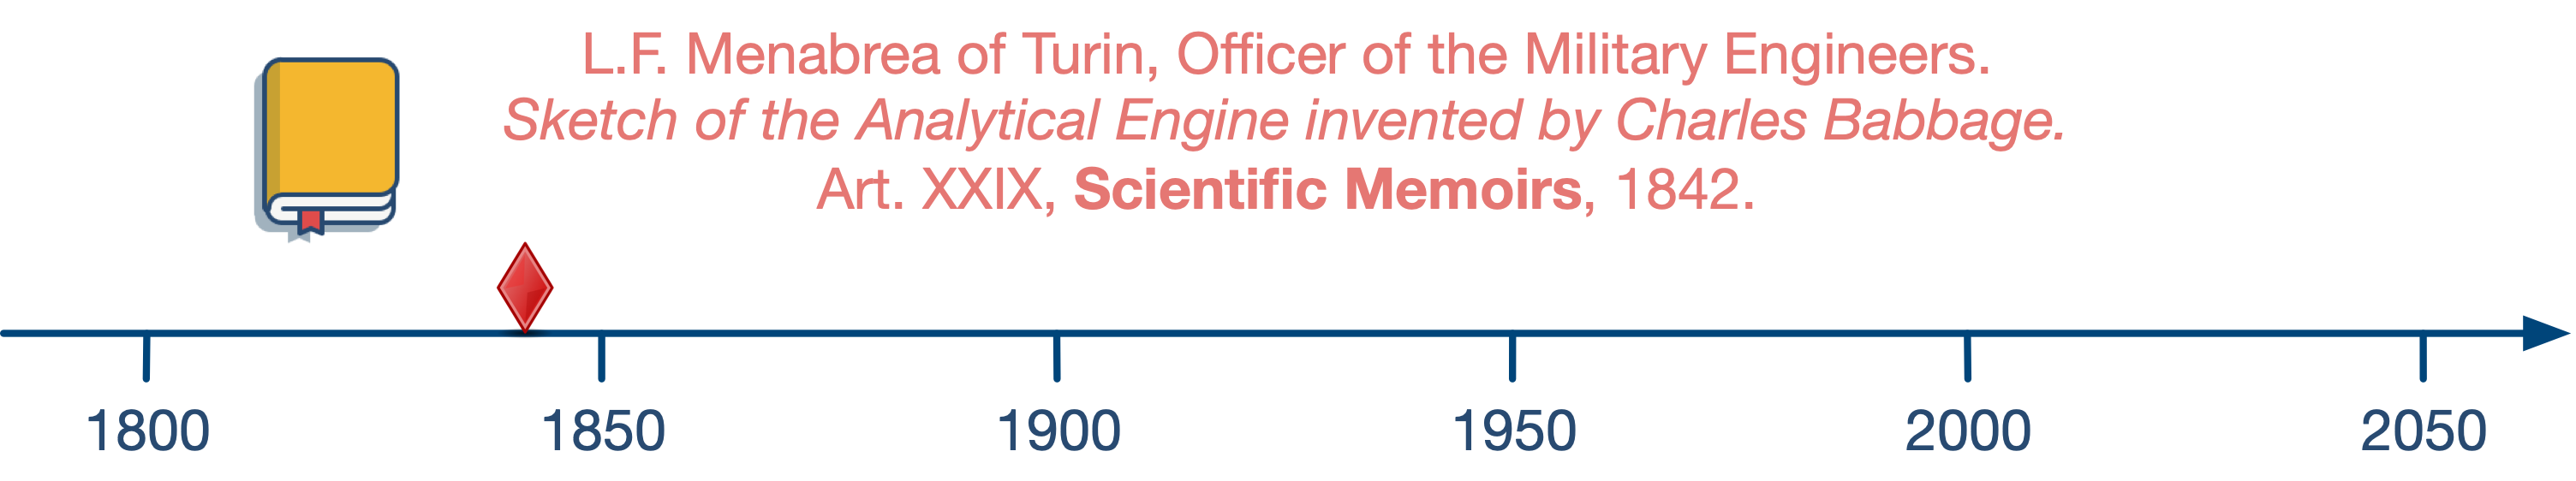
\includegraphics[width=\textwidth]{AI-timeline-1842-alt.png}
                \end{figure}
            \end{minipage}
            \\\vspace*{3pt}
	    	\begin{minipage}[t]{\textwidth}
				\begin{minipage}[t]{0.6\textwidth}
	    			\begin{itemize}[leftmargin=10pt,align=right]
						\onslide<2->\item[\alert{\faArrowCircleRight}] Mente visionaria dietro la \alert{macchina analitica di Babbage}
						\onslide<3->\item[\alert{\faArrowCircleRight}] Definì per prima il concetto di \alert{ricorsione algoritmica} nel caso della computazione dei numeri di Bernoulli
						\onslide<4->\item[\alert{\faArrowCircleRight}] Contributo dimostrato solo un secolo dopo (Harvard Mark I ideato da Howard Aiken e finanziato da IBM nel 1944)
						\onslide<5->\item[\alert{\faArrowCircleRight}] Macchina di calcolo che si potesse programmare e riprogrammare per eseguire diverse funzioni (\alert{macchina universale})
					\end{itemize}
            	\end{minipage}
            	%
				\onslide<1->
            	\begin{minipage}[t]{0.4\textwidth}
                	\centering
                	\begin{figure}[ht]
                    	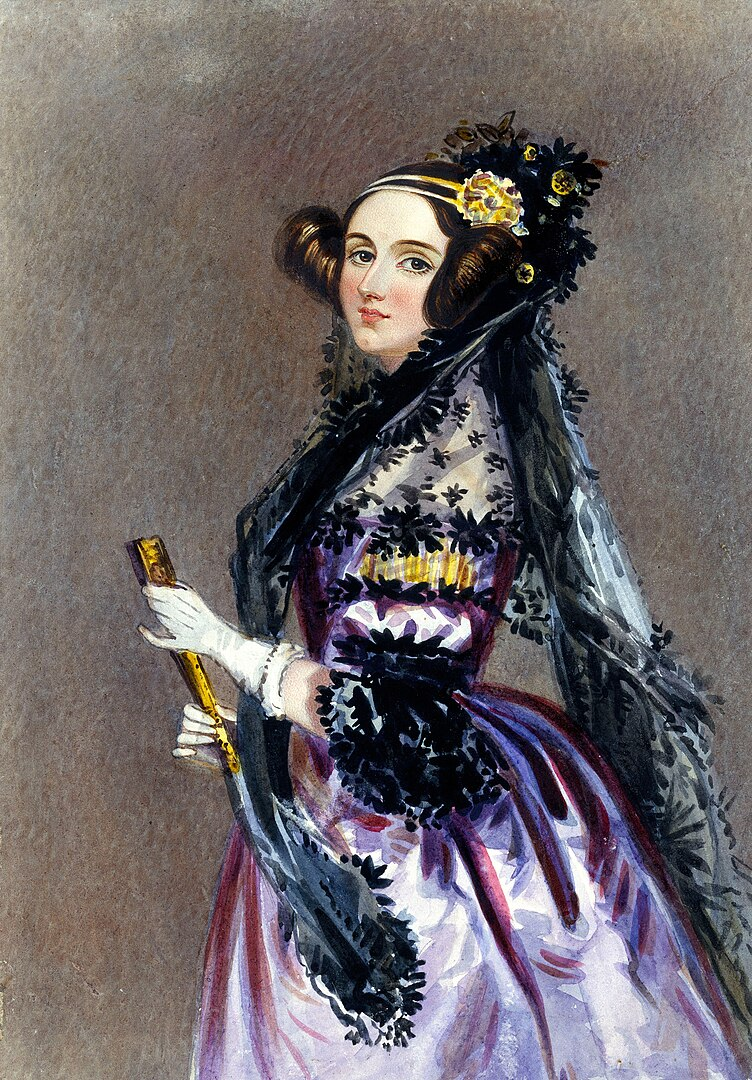
\includegraphics[width=.6\textwidth]{752px-Ada_Lovelace_portrait.jpg}
                    	{\tiny\\Augusta Ada Byron Lovelace\\\vspace*{-1pt}\textit{\textcopyright Wikimedia Creative Commons}}
                	\end{figure}
            	\end{minipage}
	    	\end{minipage}
	}
\end{frame}
%
\begin{frame}[t,fragile] \frametitle{Nascita della AI}
	{\scriptsize
		\onslide<1->
            \framesubtitle{Dalla macchina al \textit{test} di Turing}
            \vspace*{-15pt}
            \begin{minipage}[t]{\textwidth}
             	\begin{figure}[ht]
                    \centering
                    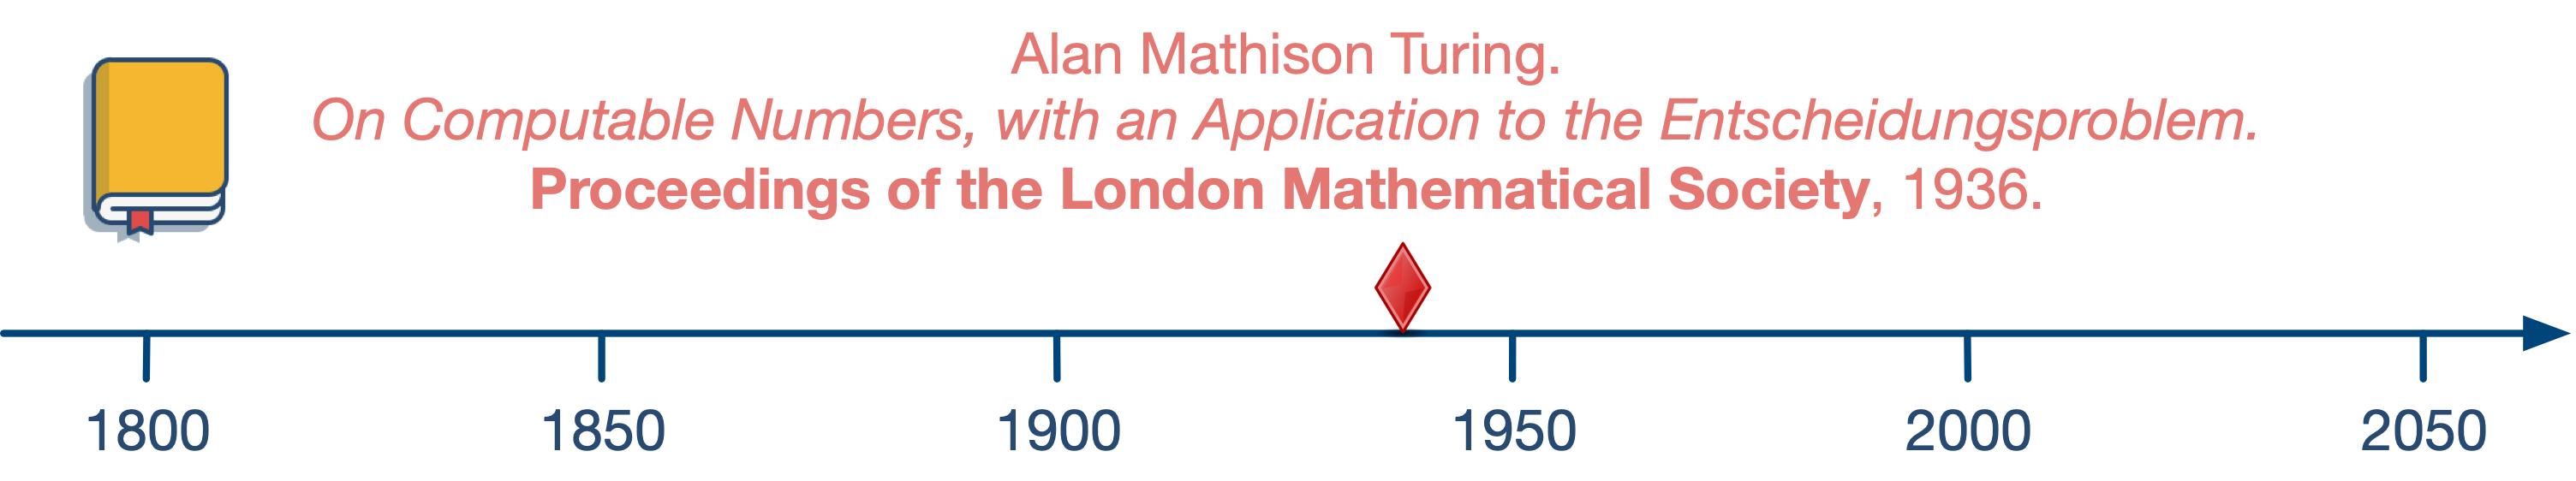
\includegraphics[width=\textwidth]{AI-timeline-1936-alt.png}
                \end{figure}
            \end{minipage}
            \\\vspace*{3pt}
	    	\begin{minipage}[t]{\textwidth}
				\begin{minipage}[t]{0.6\textwidth}
	    			\begin{itemize}[leftmargin=10pt,align=right]
						\onslide<2->\item[\alert{\faArrowCircleRight}] Modello di calcolo astratto in grado di eseguire sequenze di istruzioni (\alert{algoritmi}) attraverso lettura e scrittura su nastro e regole (simulazione del processo di calcolo umano)
						\onslide<3->\item[\alert{\faArrowCircleRight}] Ogni funzione computabile è Turing-computabile
                    	\onslide<4->\begin{itemize}[leftmargin=10pt,align=right]
							\item[\alert{\faArrowCircleRight}] Tutto ciò che una macchina di calcolo reale può computare è calcolabile da una macchina di Turing
							\item[\alert{\faArrowCircleRight}] \textit{Standard} per definire la complessità di un algoritmo, la decidibilità o meno di un problema da risolvere
						\end{itemize}
                    	\onslide<5->\item[\alert{\faArrowCircleRight}] Ultimo \alert{\textbf{no}} al \alert{problema della decidibilità} di Hilbert (1928)
						\begin{itemize}[leftmargin=10pt,align=right]
							\item[\alert{\faArrowCircleRight}] \textit{Esiste una procedura meccanica in grado di decidere in tempo finito se, nell'ambito di una teoria matematica, una data affermazione sia vera o falsa?}
						\end{itemize}
					\end{itemize}
            	\end{minipage}
				%
				\onslide<1->
            	\begin{minipage}[t]{0.4\textwidth}
                	\centering
                	\begin{figure}[ht]
						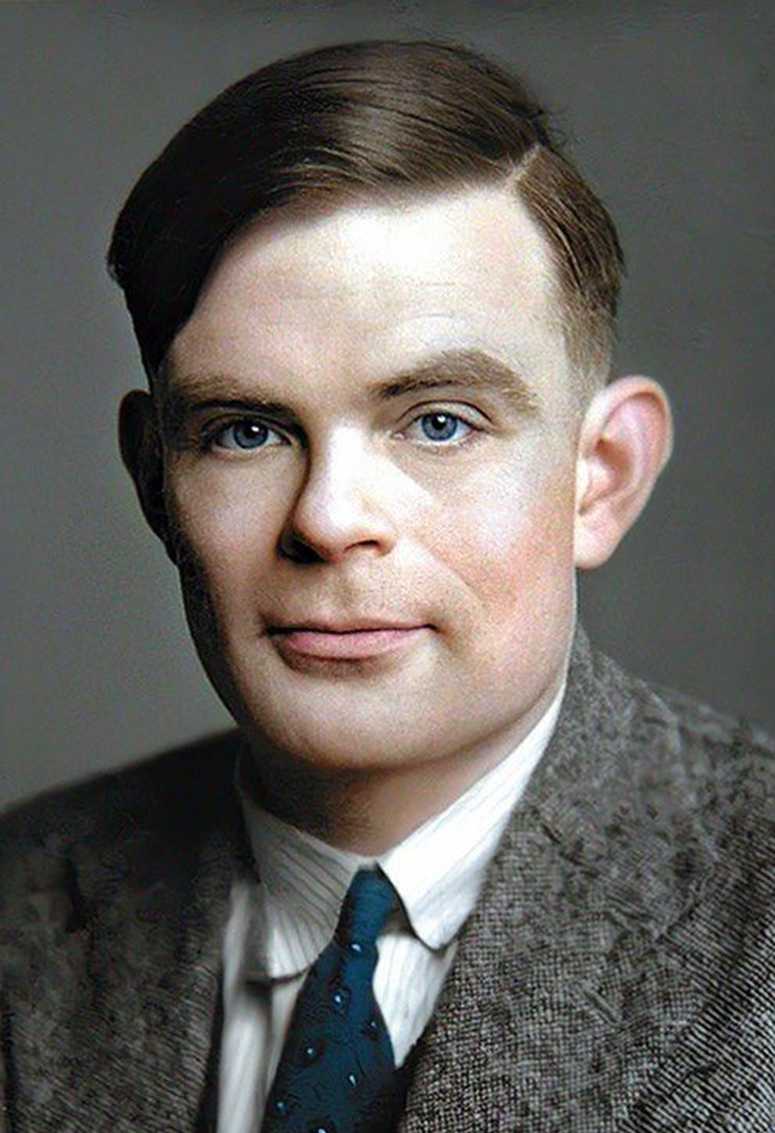
\includegraphics[width=.6\textwidth]{alan-turing-color.png}
						{\tiny\\Alan Mathison Turing\\\vspace*{-1pt}\textit{\textcopyright Elcorreo.com}}
                	\end{figure}
            	\end{minipage}
	    	\end{minipage}
	}
\end{frame}
%
\subsection{Test di Turing}
\label{subsec:turing_test}
%
\begin{frame}[t,fragile] \frametitle{Nascita della AI}
    {\scriptsize
    \onslide<1->
        \framesubtitle{Dalla macchina al \textit{test} di Turing}
        \vspace*{-15pt}
	    \begin{minipage}[t]{\textwidth}
		    \begin{figure}[ht]
			    \centering
			    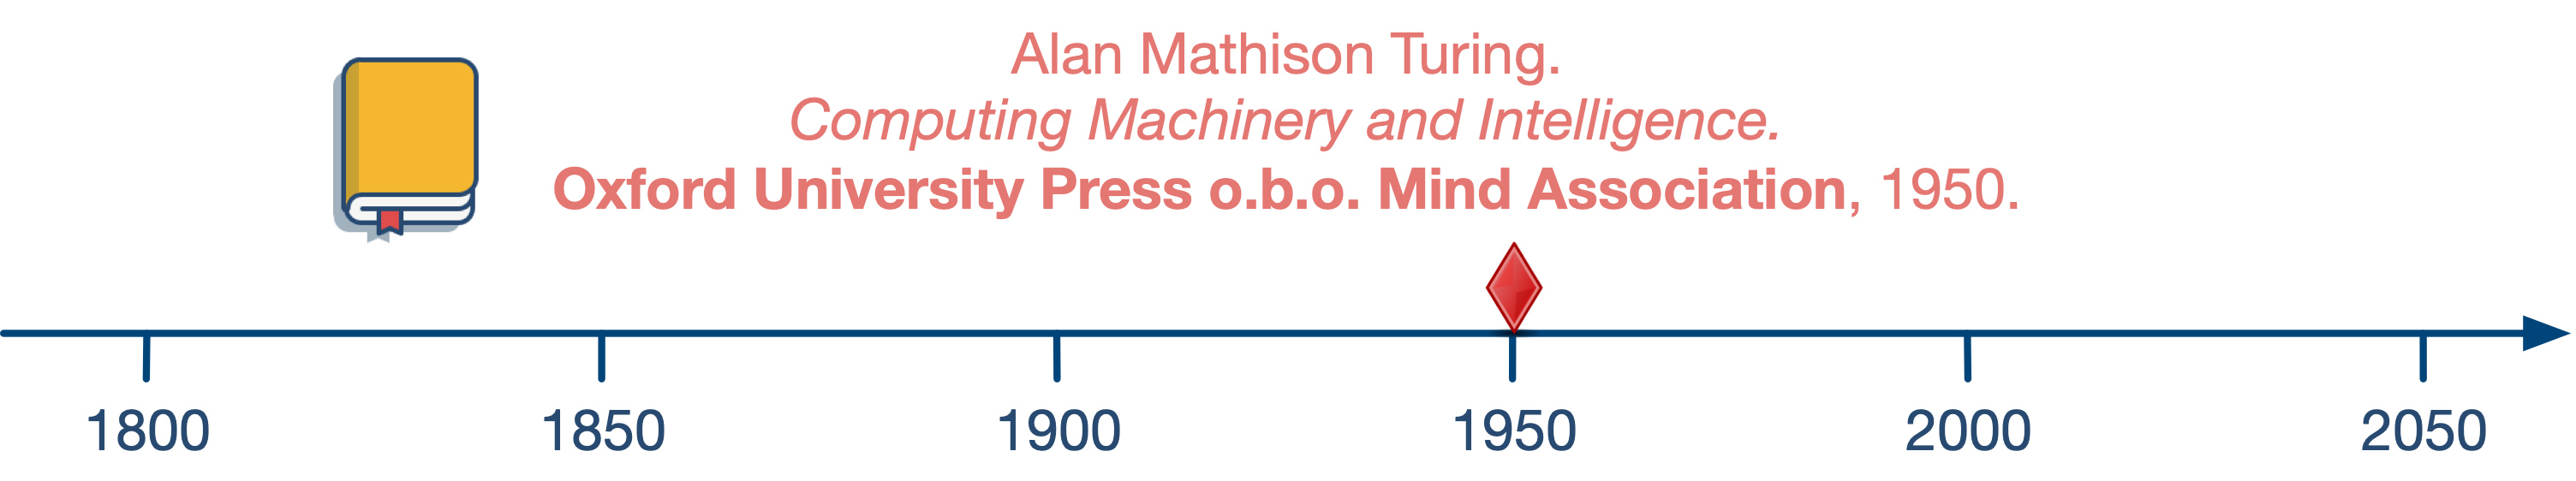
\includegraphics[width=\textwidth]{AI-timeline-1950-alt.png}
		    \end{figure}
	    \end{minipage}
	    \\\vspace*{3pt}
	    \begin{minipage}[t]{\textwidth}
		    \begin{minipage}[t]{0.6\textwidth}
			    \begin{itemize}[leftmargin=10pt,align=right]
				    \onslide<2->\item[\alert{\faArrowCircleRight}] Propone il primo esperimento per valutare l'intelligenza di una macchina (\alert{\textit{test} di Turing} o \alert{\textit{Imitation Game}})
				    \onslide<3->\begin{itemize}[leftmargin=10pt,align=right]
						\item[\alert{\faArrowCircleRight}] Una macchina e un umano in due stanze separate
						\item[\alert{\faArrowCircleRight}] Un arbitro umano pone delle domande a entrambi per definire chi è l'umano dei due
						\item[\alert{\faArrowCircleRight}] Se l'arbitro non riesce a determinare la natura degli interlocutori, allora la macchina ha raggiunto un comportamento intelligente
				    \end{itemize}
				    \onslide<4->\item[\alert{\faArrowCircleRight}] Impone la comprensione del linguaggio come \alert{condizione sufficiente} dell'intelligenza
					\begin{itemize}[leftmargin=10pt,align=right]
						\item[\alert{\faArrowCircleRight}] Ipotesi largamente criticata
					\end{itemize}
					\begin{center}
						\hyperlink{subsec:searle}{\color{venis-faithful-yellow}\faExternalLinkSquare\ Maggiori informazioni}
					\end{center}
			    \end{itemize}
		    \end{minipage}
		    %
		    \onslide<1->
		    \begin{minipage}[t]{0.4\textwidth}
			    \centering
			    \begin{figure}[ht]
				    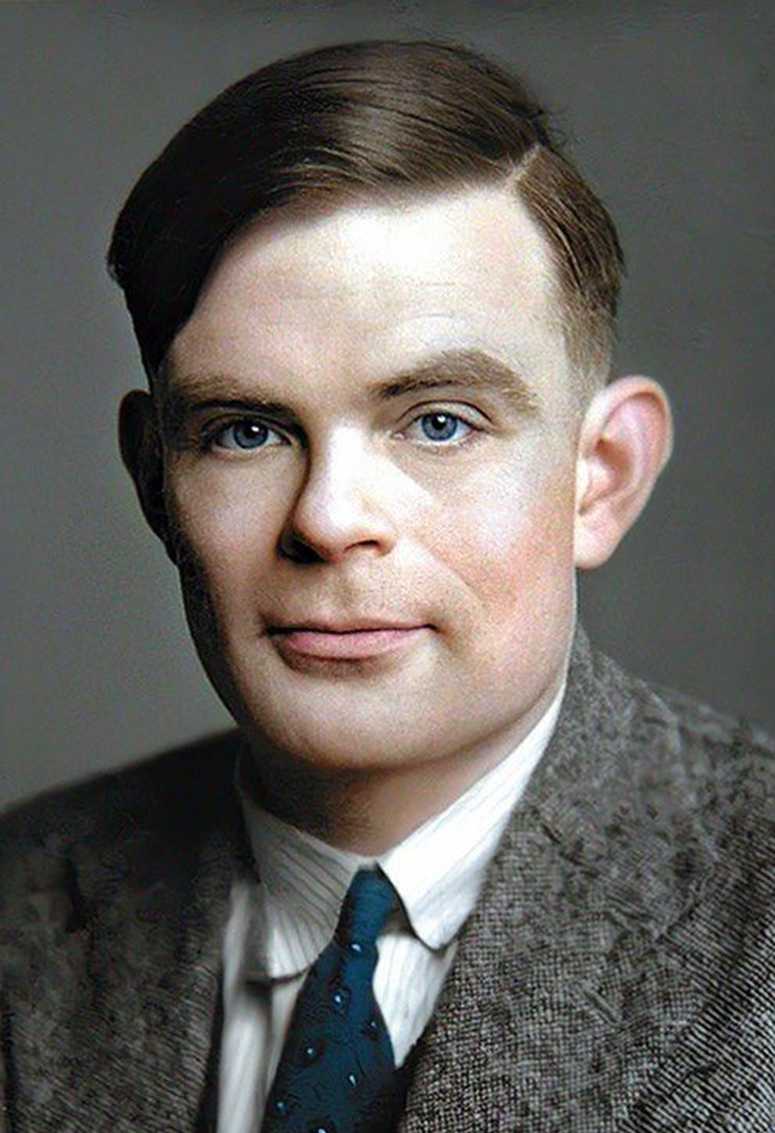
\includegraphics[width=.6\textwidth]{alan-turing-color.png}
				    {\tiny\\Alan Mathison Turing\\\vspace*{-1pt}\textit{\textcopyright Elcorreo.com}}
			    \end{figure}
		    \end{minipage}
	    \end{minipage}
    }
\end{frame}
%
\begin{frame}[t,fragile] \frametitle{Nascita della AI}
{\scriptsize
	\onslide<1->
		\framesubtitle{\textit{Habemus} AI!}
		\vspace*{-15pt}
		\begin{minipage}[t]{\textwidth}
			\begin{figure}[ht]
				\centering
				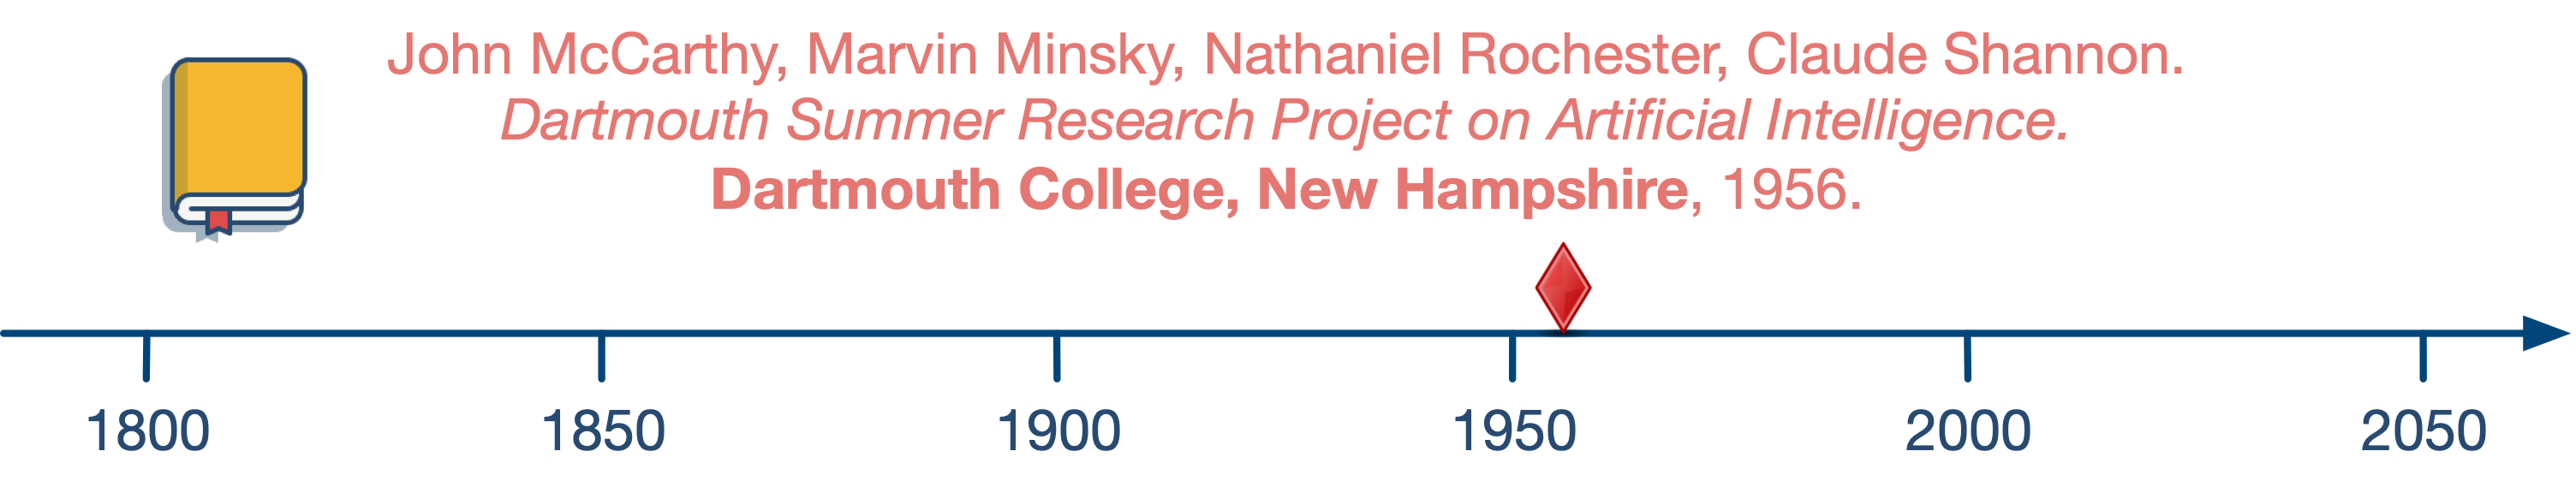
\includegraphics[width=\textwidth]{AI-timeline-1956-2-alt.png}
			\end{figure}
		\end{minipage}
	\only<1|handout:0>{
	\begin{minipage}[t]{.4\textwidth}
		\vspace*{10pt}
		\begin{minipage}[t]{0.45\textwidth}
			\centering
			\begin{figure}[ht]
				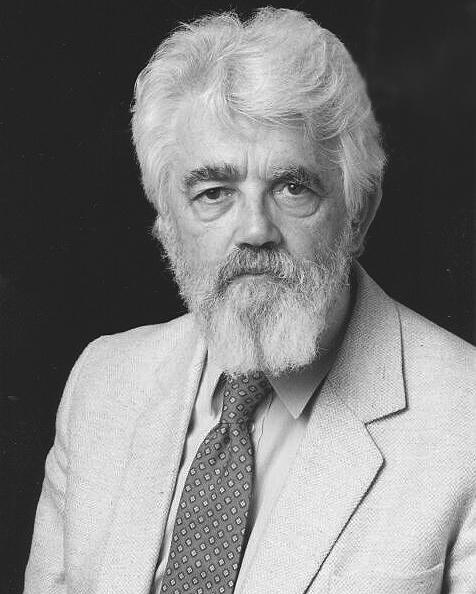
\includegraphics[width=.73\textwidth]{John-McCarthy.jpg}
				{\tiny\\John McCarthy\\\vspace*{-1pt}\textit{\textcopyright Naukas}}
			\end{figure}
		\end{minipage}
		\hfill
		\begin{minipage}[t]{0.45\textwidth}
			\centering
			\begin{figure}[ht]
				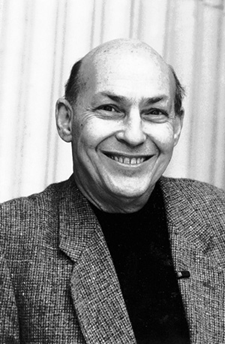
\includegraphics[width=.6\textwidth]{Marvin-Misky.png}
				{\tiny\\Marvin Minsky\\\vspace*{-1pt}\textit{\textcopyright Donna Coveny}}
			\end{figure}
		\end{minipage}
		\begin{minipage}[t]{0.45\textwidth}
			\centering
			\begin{figure}[ht]
				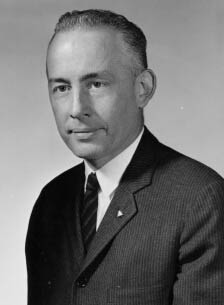
\includegraphics[width=.68\textwidth]{Nathaniel-Rochester.jpeg}
				{\tiny\\Nathaniel Rochester\\\vspace*{-1pt}\textit{\textcopyright dmodha}}
			\end{figure}
		\end{minipage}
		\hfill
		\begin{minipage}[t]{0.45\textwidth}
			\centering
			\begin{figure}[ht]
				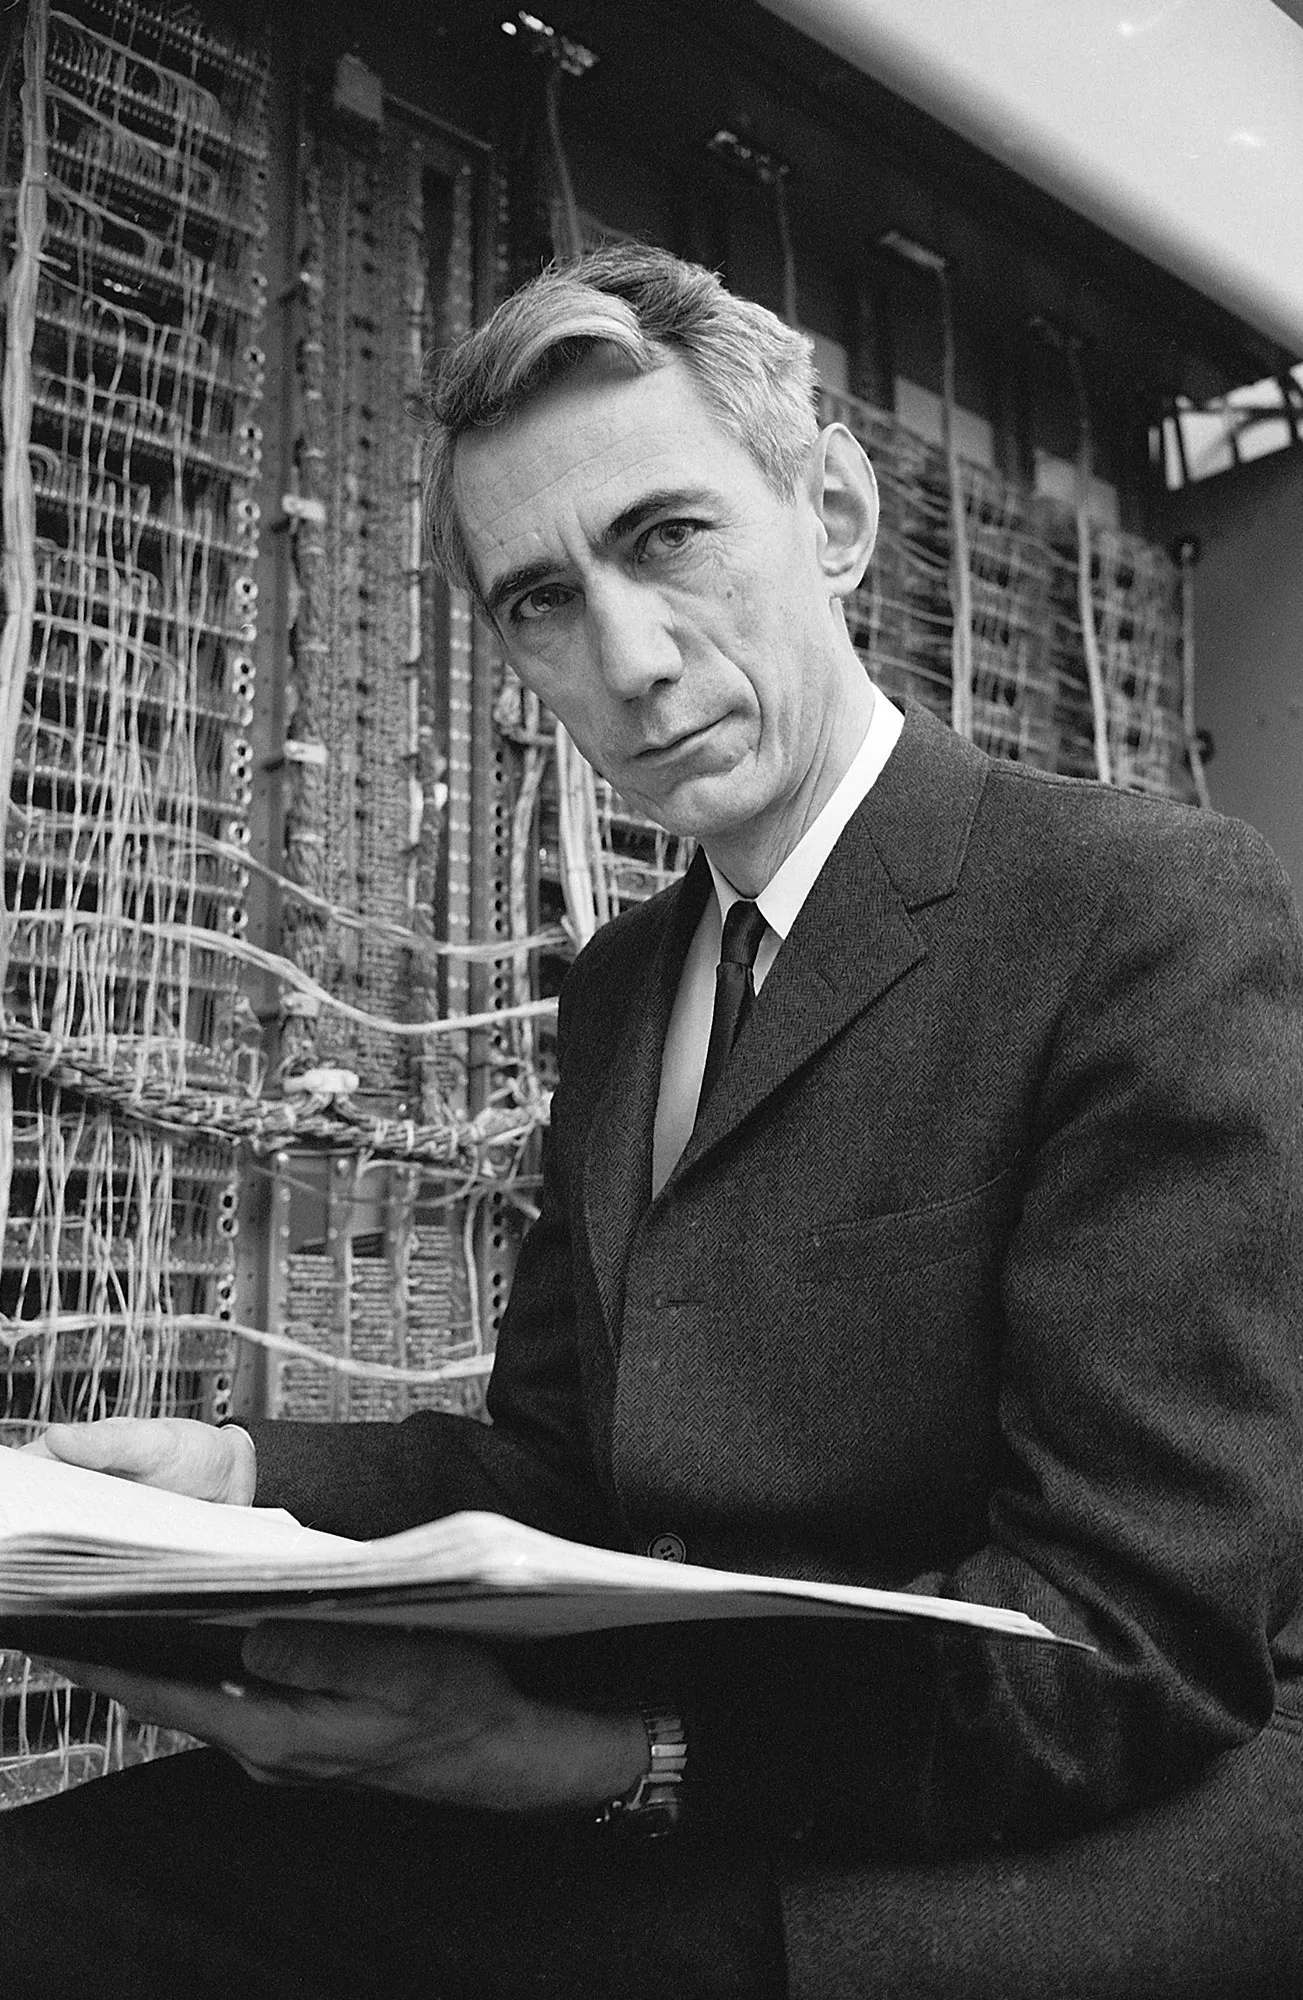
\includegraphics[width=.6\textwidth]{Roberts-Claude-Shannon.png}
				{\tiny\\Claude Shannon\\\vspace*{-1pt}\textit{\textcopyright Alfred Eisenstaedt}}
			\end{figure}
		\end{minipage}
	\end{minipage}
	}
	\only<2|handout:1>{
	\begin{minipage}[t]{.4\textwidth}
		\vspace*{10pt}
		\begin{minipage}[t]{0.9\textwidth}
			\centering
			\begin{figure}[ht]
				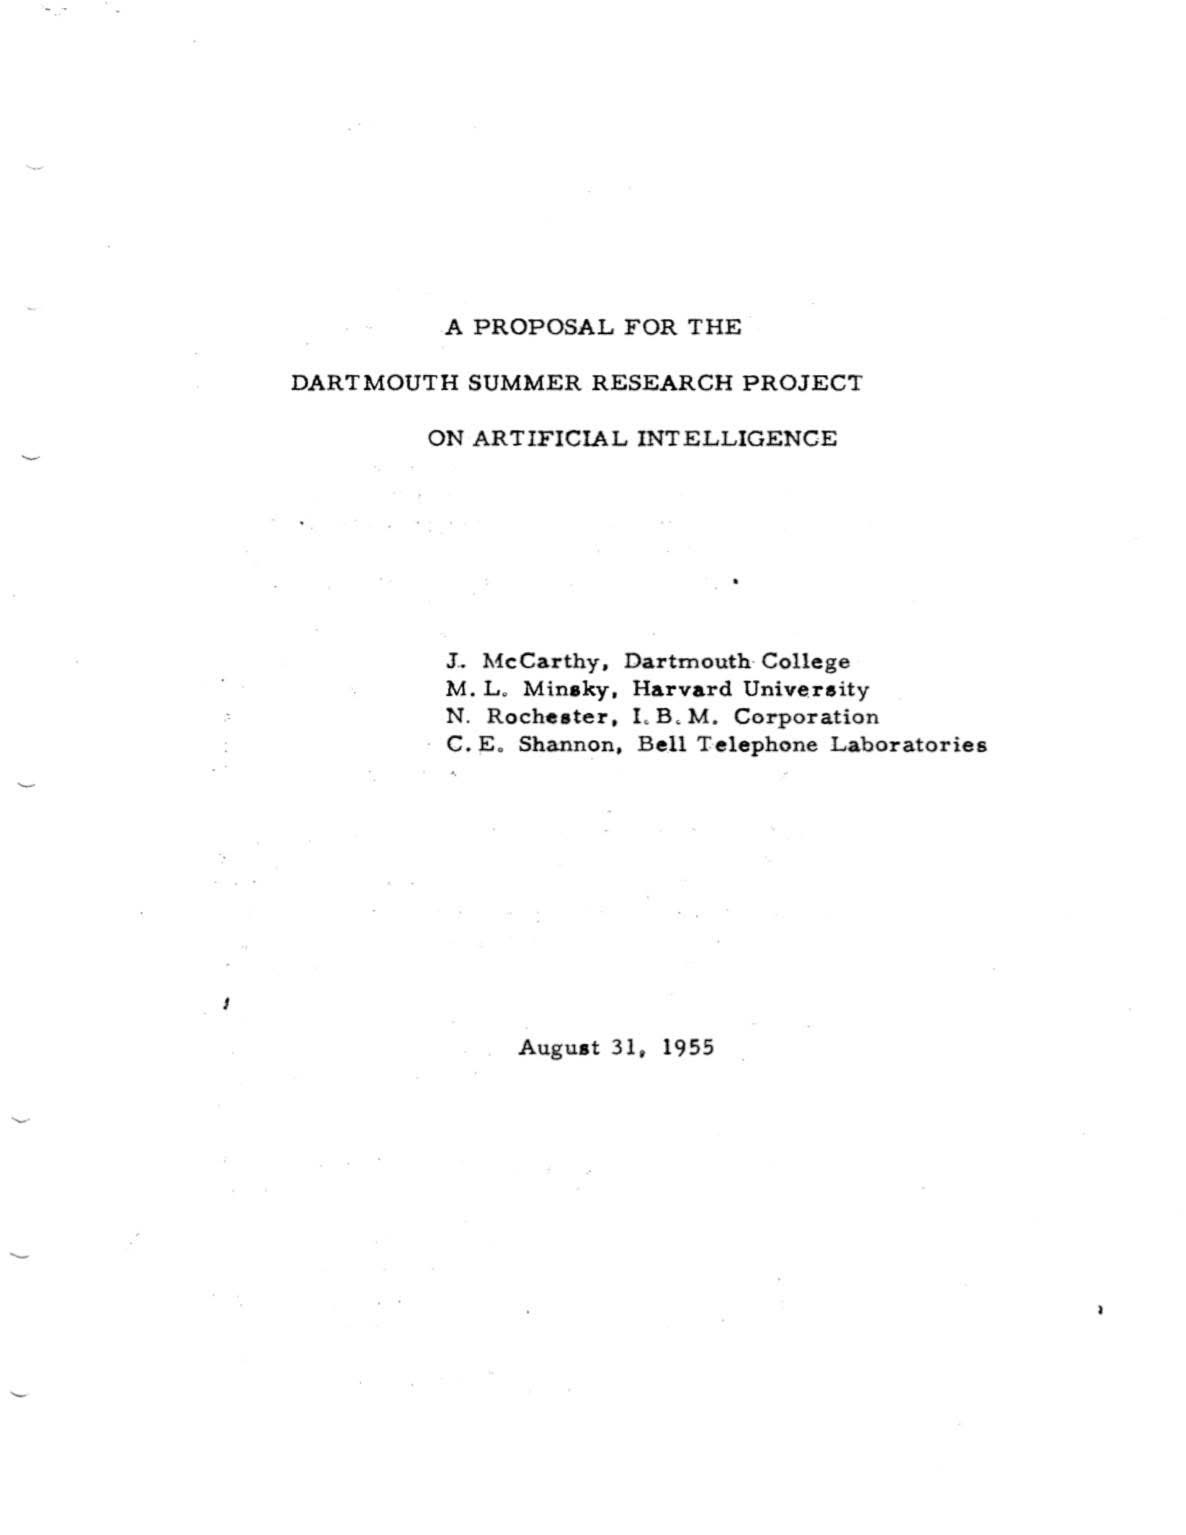
\includegraphics[width=.8\textwidth, frame]{IMG_0672.JPG}
				{\tiny\\Frontespizio\\\vspace*{-1pt}\textit{\textcopyright Naukas}}
			\end{figure}
		\end{minipage}
	\end{minipage}
	}
	\hfill
	\onslide<2->	
		\begin{minipage}[t]{.55\textwidth}
			\renewcommand{\epigraphsize}{\scriptsize}
			\setlength{\afterepigraphskip}{0pt}
			\setlength{\beforeepigraphskip}{10pt}
			\setlength{\epigraphwidth}{\textwidth}
			\epigraph{\textit{Proponiamo che uno studio di 2 mesi, condotto da 10 persone, sull'\alert{intelligenza artificiale} venga svolto durante l'estate del 1956 presso il Dartmouth College di Hanover, nel New Hampshire. Lo studio dovrà procedere sulla base dell'ipotesi che ogni aspetto dell'apprendimento o qualunque altra caratteristica dell'intelligenza possa, in linea di principio, essere descritto con tanta precisione da consentire la costruzione di una macchina capace di simularlo. Si tenterà di scoprire come far sì che le macchine usino il linguaggio, formino astrazioni e concetti, risolvano tipi di problemi attualmente riservati agli esseri umani e siano in grado di migliorare se stesse. [\ldots]
}}{\textit{Summer School Project}, estratto, \textbf{Dartmouth, 1956}\\Traduzione: \textit{\textcopyright ChatGPT}}
		\end{minipage}%
	}
\end{frame}
%
\begin{frame}[t,fragile] \frametitle{Cronistoria della AI}
	\framesubtitle{1950-1975: dalle stelle\ldots}
	\vspace*{-15pt}
	\begin{figure}[ht]
        	\centering
        	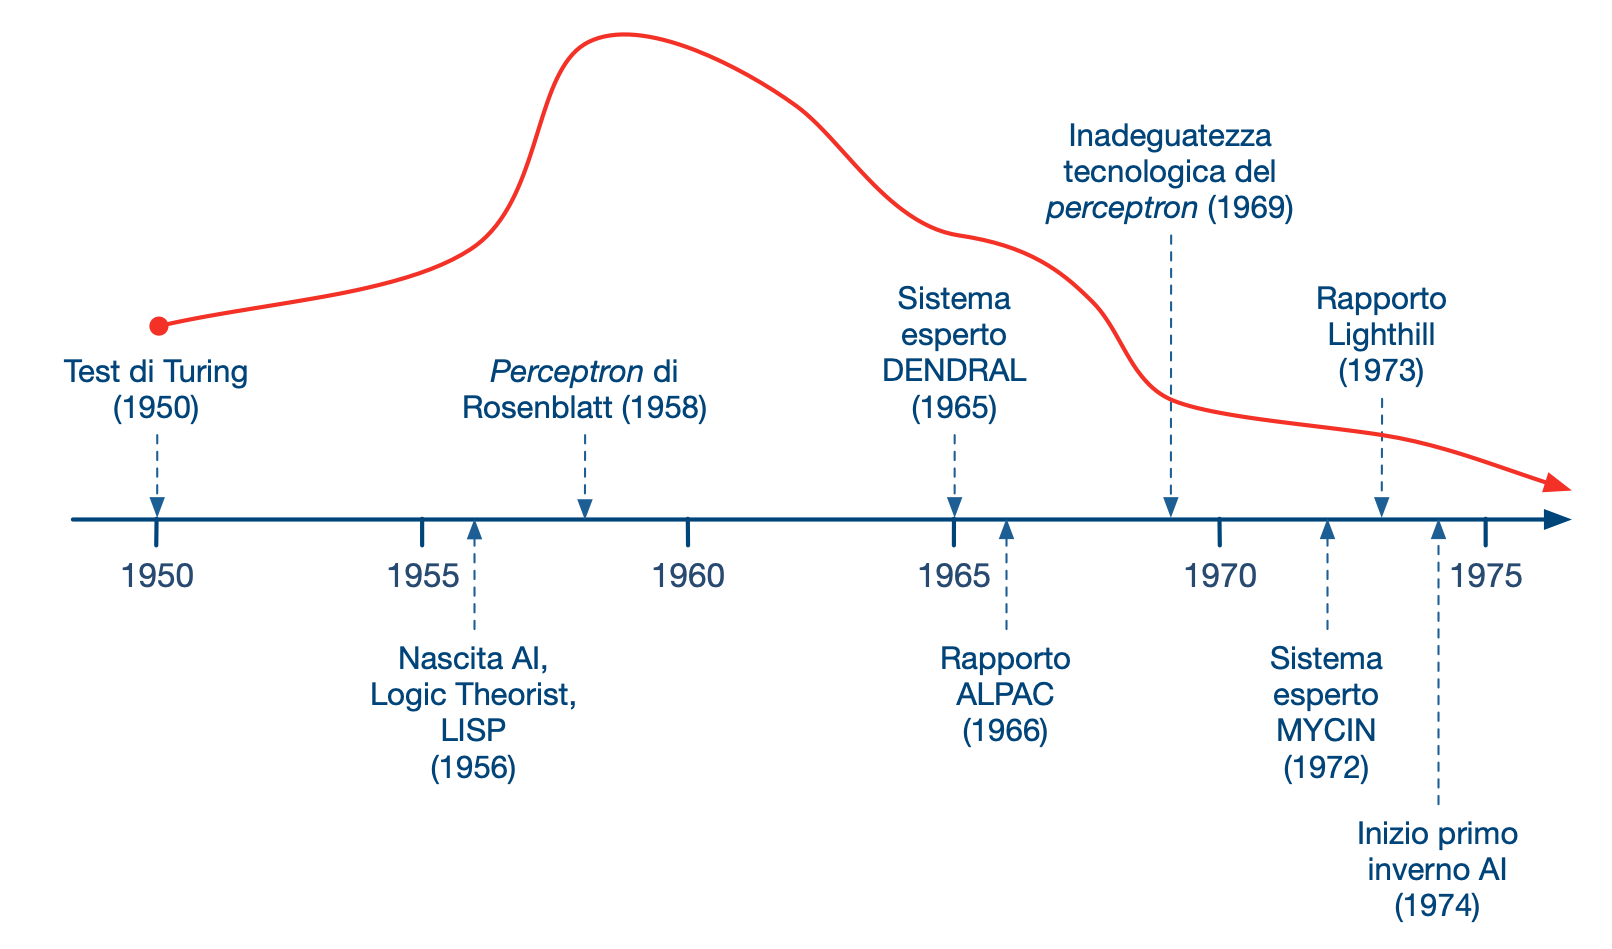
\includegraphics[width=\textwidth]{AI-rollercoaster-1.png}
    \end{figure}
	\begin{flushright}
    	\vspace*{-10pt}
        {\tiny\textit{\textcopyright Simone Scannapieco. I valori delle ordinate sono puramente indicativi.}}
	\end{flushright}
\end{frame}
%
\subsection{Caduta della AI}
\label{subsec:ai_fall}
%
\begin{frame}[t,fragile] \frametitle{Cronistoria della AI}
	\framesubtitle{1950-1975: cause del primo inverno AI}
	{\small
	\begin{itemize}[leftmargin=10pt,align=right]
	\only<1|handout:1>{\item[\alert{\faArrowCircleRight}] \alert{Aspettative esagerate:} la ricerca in AI fece previsioni troppo audaci sulle capacità dell'AI che non si sono materializzate}
	\only<2|handout:2>{\item[\alert{\faArrowCircleRight}] \alert{Limitazioni tecniche:} potenza di calcolo e algoritmi insufficienti per risolvere problemi complessi del mondo reale (\textit{perceptron})}
	\only<3|handout:3>{\item[\alert{\faArrowCircleRight}] \alert{Esplosione combinatoria:} molti problemi di AI affrontavano una crescita esponenziale della complessità all'aumentare delle dimensioni dell'\textit{input}}
	\only<4|handout:4>{\item[\alert{\faArrowCircleRight}] \alert{Rapporto ALPAC (1966):} infattibilità tecnologica della traduzione automatica, con relativo tagli dei finanziamenti
	         \item[\alert{\faArrowCircleRight}] \alert{Rapporto Lighthill (1973):} critica feroce agli obiettivi AI non realizzati; i tagli in UK causarono un effetto domino a livello mondiale (DARPA in USA)}
	\only<5|handout:5>{\item[\alert{\faArrowCircleRight}] \alert{Paradosso di Moravec (1988):} più il compito è semplice per un umano, più è difficile per una macchina da emulare (e viceversa)}
	\only<6|handout:6>{\item[\alert{\faArrowCircleRight}] \alert{Crollo dei sistemi esperti:} \normalcircled{1} troppo costosi da mantenere, \normalcircled{2} difficili da aggiornare, \normalcircled{3} non robusti di fronte a \textit{input} insoliti}
	\end{itemize}
	\vspace*{.3cm}
	\only<1|handout:1>{
	\begin{minipage}[t]{\textwidth}
		\begin{minipage}[t]{\textwidth}
			\begin{minipage}[t]{.32\textwidth}
				\renewcommand{\epigraphsize}{\scriptsize}
				\setlength{\afterepigraphskip}{0pt}
				\setlength{\beforeepigraphskip}{5pt}
				\setlength{\epigraphwidth}{0.9\textwidth}
				\epigraph{\textit{[$\ldots$] stiamo per assistere alla nascita di una macchina [$\ldots$] capace di percepire, riconoscere e identificare ciò che la circonda senza alcun addestramento o controllo da parte dell'essere umano.}}{F. Rosenblatt, Mark I Perceptron, 1958}
			\end{minipage}%
			\begin{minipage}[t]{.32\textwidth}
				\renewcommand{\epigraphsize}{\scriptsize}
				\setlength{\afterepigraphskip}{0pt}
				\setlength{\beforeepigraphskip}{5pt}
				\setlength{\epigraphwidth}{0.9\textwidth}
				\epigraph{\textit{[$\ldots$] è il primo rivale del cervello umano che sia mai stato concepito.}}{New Yorker, 1958}
			\end{minipage}%
			\begin{minipage}[t]{.32\textwidth}
				\renewcommand{\epigraphsize}{\scriptsize}
				\setlength{\afterepigraphskip}{0pt}
				\setlength{\beforeepigraphskip}{5pt}
				\setlength{\epigraphwidth}{0.9\textwidth}
				\epigraph{\textit{Ecco il cervello elettronico che insegna a se stesso.}}{The New York Times, 1958}
			\end{minipage}%
		\end{minipage}
	\end{minipage}
	}
	\only<2|handout:2>{
	\begin{minipage}[t]{\textwidth}
		\begin{minipage}[t]{0.6\textwidth}
			\centering
			\begin{figure}[ht]
				\includegraphics[width=.8\textwidth]{Perceptron-vs-neuronal-cell-scaled.png}
				{\tiny\\Neurone umano vs. \textit{perceptron}\\\vspace*{-4pt}\textit{\textcopyright Simone Scannapieco, Wikimedia Creative Commons}}
			\end{figure}
		\end{minipage}
		\hfill
		\begin{minipage}[t]{0.4\textwidth}
			\centering
			\begin{figure}[ht]
				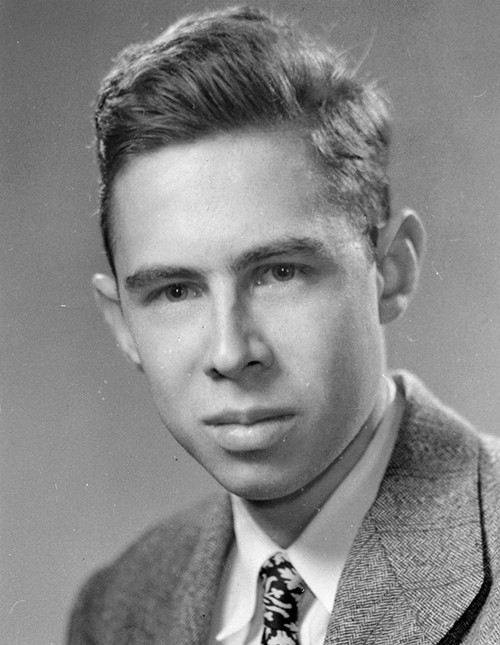
\includegraphics[width=.8\textwidth]{Frank-Rosenblatt.jpg}
				{\tiny\\Frank Rosenblatt\\\vspace*{-4pt}\textit{\textcopyright Wikimedia Creative Commons}}
			\end{figure}
		\end{minipage}
	\end{minipage}
	}
	\only<3|handout:3>{
	\begin{minipage}[t]{\textwidth}
		\begin{minipage}[t]{0.3\textwidth}
			\begin{minipage}[t]{\textwidth}
				\begin{figure}[ht]
					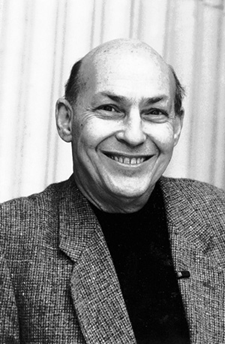
\includegraphics[width=.45\textwidth]{Marvin-Misky.png}
					{\tiny\\Marvin Minsky\\\vspace*{-4pt}\textit{\textcopyright Donna Coveny}}
				\end{figure}
			\end{minipage}
			\\
			\begin{minipage}[t]{\textwidth}
				\begin{figure}[ht]
					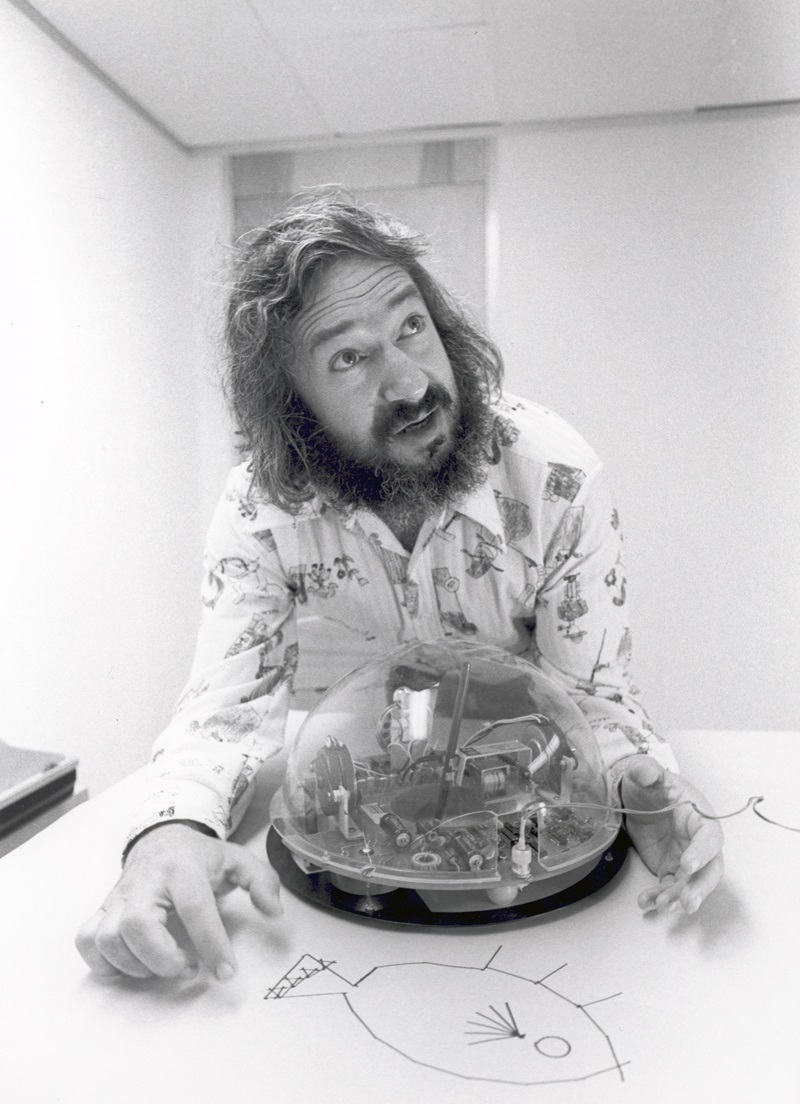
\includegraphics[width=.45\textwidth]{Seymour_Papert.jpg}
					{\tiny\\Seymour Papert\\\vspace*{-4pt}\textit{\textcopyright Matematicamente}}
				\end{figure}
			\end{minipage}
		\end{minipage}
		\hfill
		\begin{minipage}[t]{0.65\textwidth}
			\begin{itemize}[leftmargin=0pt,align=right]
			\item[\alert{\faArrowCircleRight}] Dimostrazione matematica che il \textit{perceptron} risolve operazioni elementari (\alert{linearmente separabili})
			\begin{figure}[ht]
				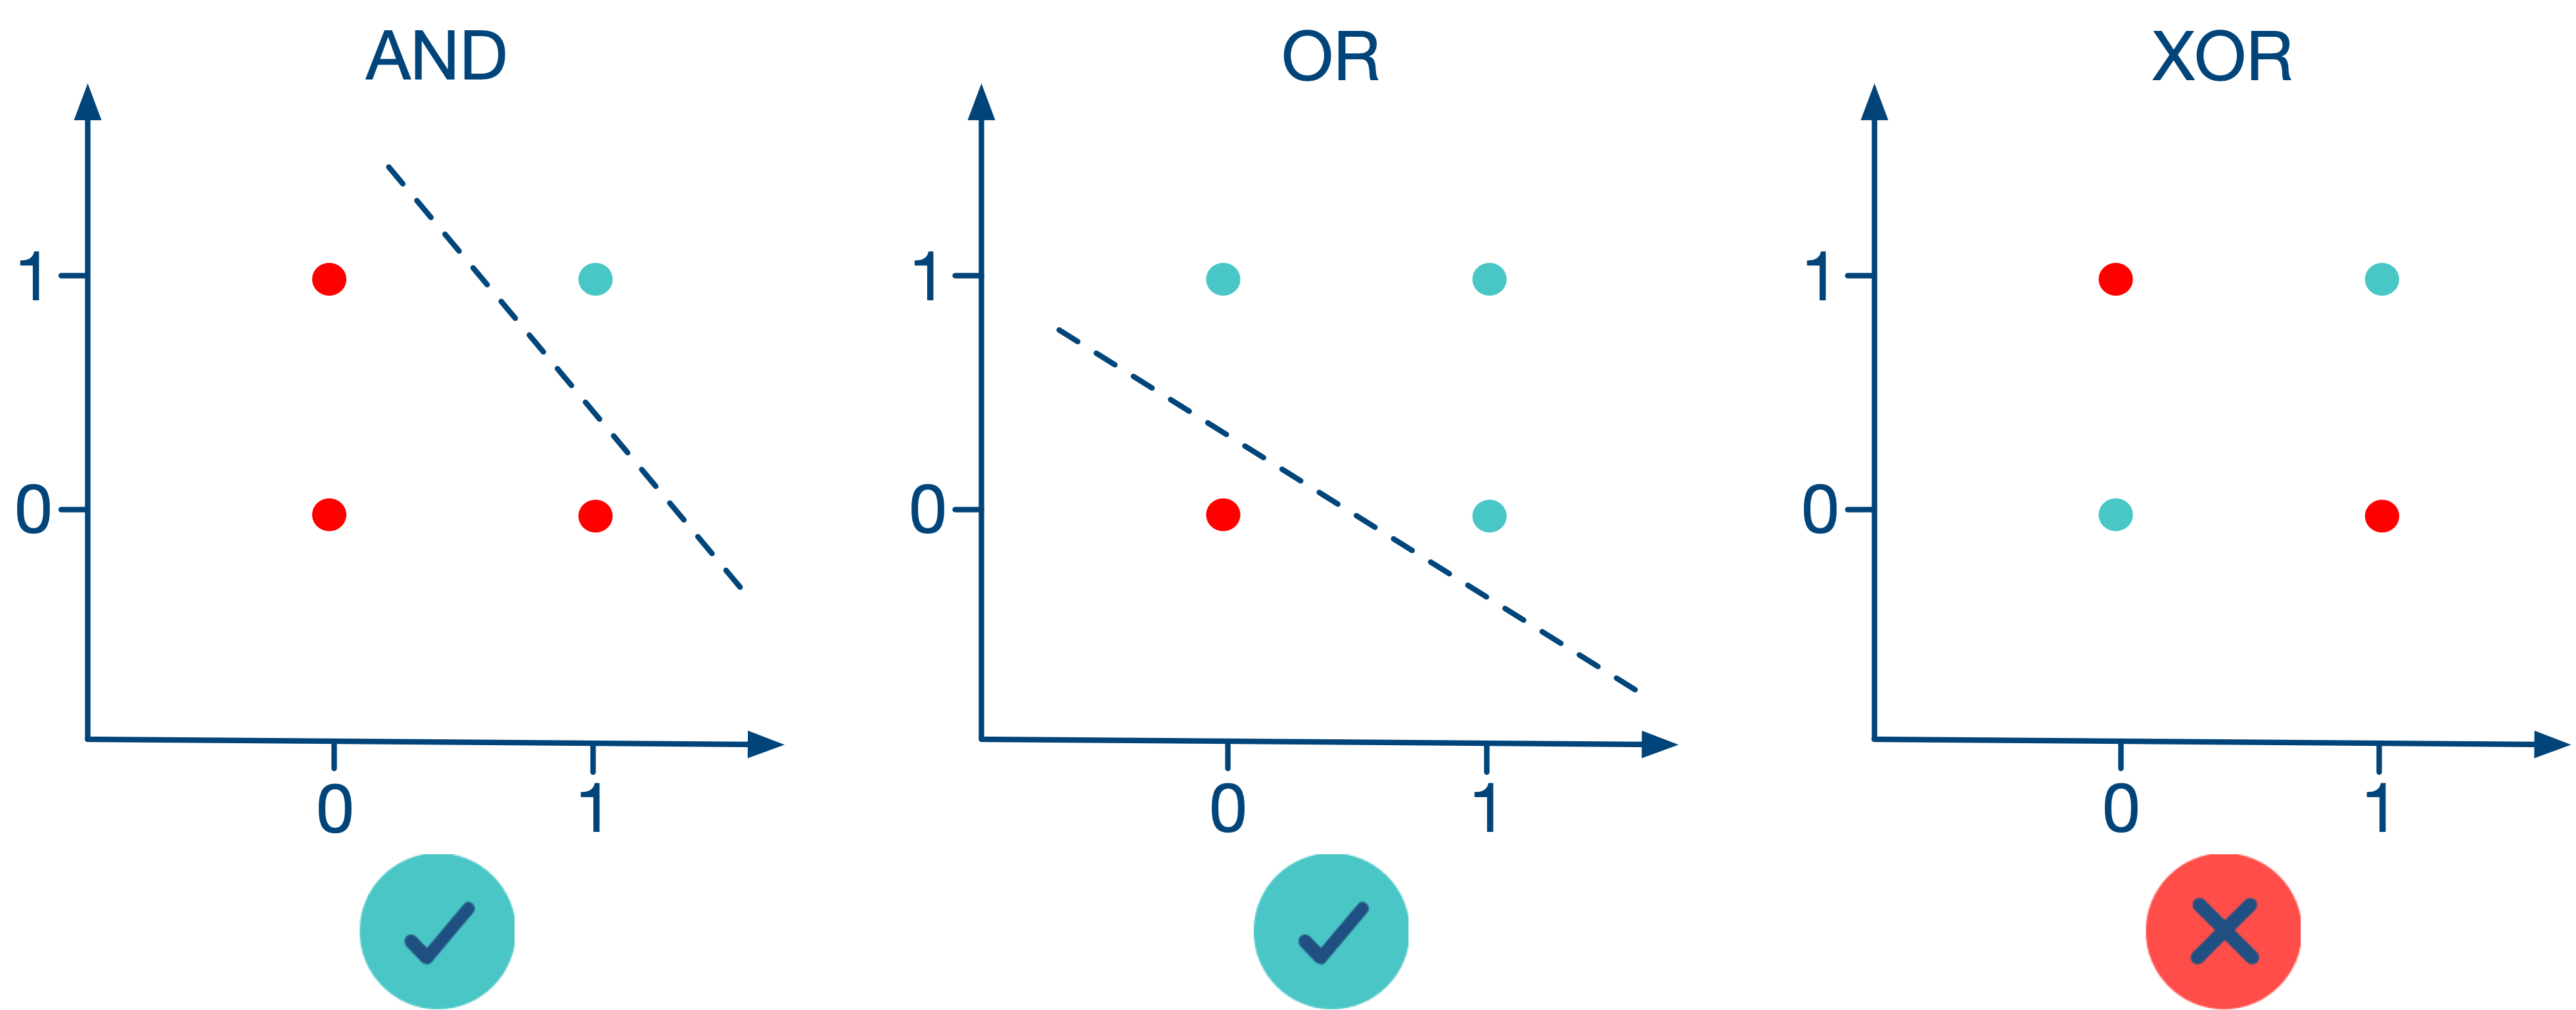
\includegraphics[width=\textwidth]{AND-OR-XOR-0.png}
			\end{figure}
			\item[\alert{\faArrowCircleRight}] Proposta teorica di \alert{aggregare più \textit{perceptron}} per risolvere problemi più complessi
		\end{itemize}
		\end{minipage}
	\end{minipage}
	}
	\only<4|handout:4>{
	\begin{minipage}[t]{\textwidth}
		\begin{minipage}[t]{0.35\textwidth}
			\begin{minipage}[t]{\textwidth}
				\begin{figure}[ht]
					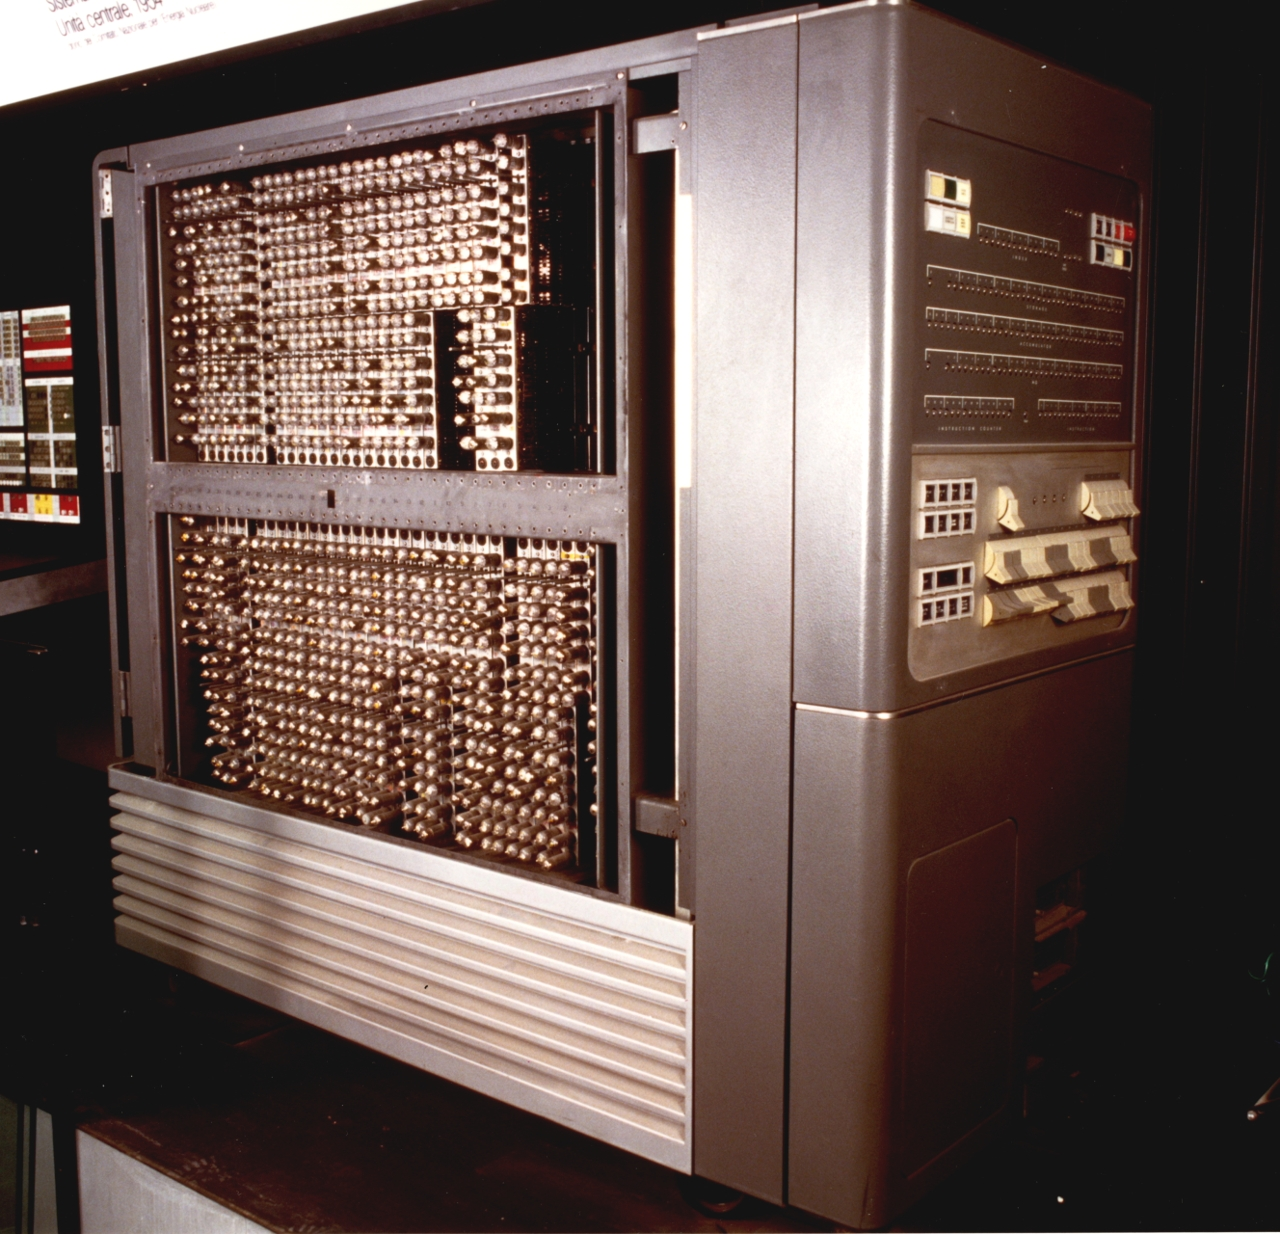
\includegraphics[width=\textwidth]{IBM-704.jpg}
					{\tiny\\Mark I Perceptron, IBM 704\\\vspace*{-4pt}\textit{\textcopyright IBM Italia}}
				\end{figure}
			\end{minipage}
		\end{minipage}
		\hfill
		\begin{minipage}[t]{0.6\textwidth}
			{\scriptsize
			\begin{table}
				%% increase table row spacing, adjust to taste
				\setlength{\tabcolsep}{0pt}
				\renewcommand{\arraystretch}{1.3}
				\centering
				\begin{tabular}{p{3cm}p{3cm}}
					\toprule
					\textbf{Nome progetto} & Mark I Perceptron\\
					\textbf{Finanziatore} & Marina USA\\
					\textbf{Dimensioni (H $\times$ L $\times$ P)}  & 167 $\times$ 176 $\times$ 80 cm\\
					\textbf{Peso} & > 5 Tonnellate\\
					\textbf{Investimento}  & 1.2 Milioni USD (stimato)\\
					\textbf{Esperimenti} & Marcatura schede perforate\newline
					 Quadrati vs cerchi (99.8\%)\newline
					 Quadrati vs diamanti (100\%)\newline
					 Lettera X vs E (100\%)\newline
					 Lettera E vs F (80\%) \\
					\bottomrule
				\end{tabular}
			\end{table}
			}
		\end{minipage}
	\end{minipage}
	}
	\only<5|handout:5>{
	\begin{minipage}[t]{\textwidth}
		\begin{minipage}[b]{0.4\textwidth}
			\begin{figure}[ht]
				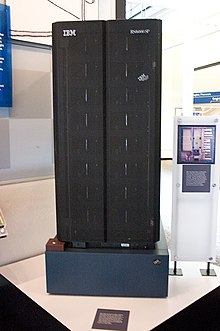
\includegraphics[height=4.5cm,keepaspectratio]{Deep_Blue.jpg}
				{\tiny\\La macchina batte l'umano\\\textbf{Garry Kasparow vs Deep Blue (1996-1997)}\\\vspace*{-4pt}\textit{\textcopyright IBM}}
			\end{figure}
		\end{minipage}
		\hfill
		\begin{minipage}[b]{0.55\textwidth}
			\centering
			%\simplemedia[showGUI=false,autoplay=true]{\vbox to 4.5cm{\vfil\hbox to 5.5cm{}\vfil}}{video/Humanoid-Robot-Goes-Berserk-During-Test-Run.mp4}{video/mp4}
			\presentvideo{Humanoid-Robot-Goes-Berserk-During-Test-Run-thumbnail.png}{video/Humanoid-Robot-Goes-Berserk-During-Test-Run.mp4}
			{\tiny\\\href{https://www.youtube.com/watch?v=m8VUrP5O048}{\faExternalLinkSquare\ Humanoid Robot Goes Berserk During Test Run}\\\textbf{Unitree H1, China (2025)}\\\vspace*{-4pt}\textit{\textcopyright QuantumEdge Vortex - Youtube}}
		\end{minipage}
	\end{minipage}
	}
	\only<6|handout:6>{
	\begin{minipage}[t]{\textwidth}
		\begin{minipage}[b]{0.25\textwidth}
			\centering
			\begin{figure}[ht]
				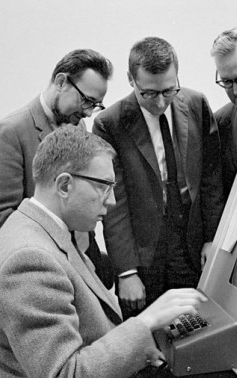
\includegraphics[height=3.5cm,keepaspectratio]{Edward-Feigenbaum-crop.png}
				{\tiny\\Edward Feigenbaum\\\textbf{Sistema DENDRAL (1965)}\\\vspace*{-4pt}\textit{\textcopyright Klondike.ai}}
			\end{figure}
		\end{minipage}
		\hfill
		\begin{minipage}[b]{0.25\textwidth}
			\centering
			\begin{figure}[ht]
				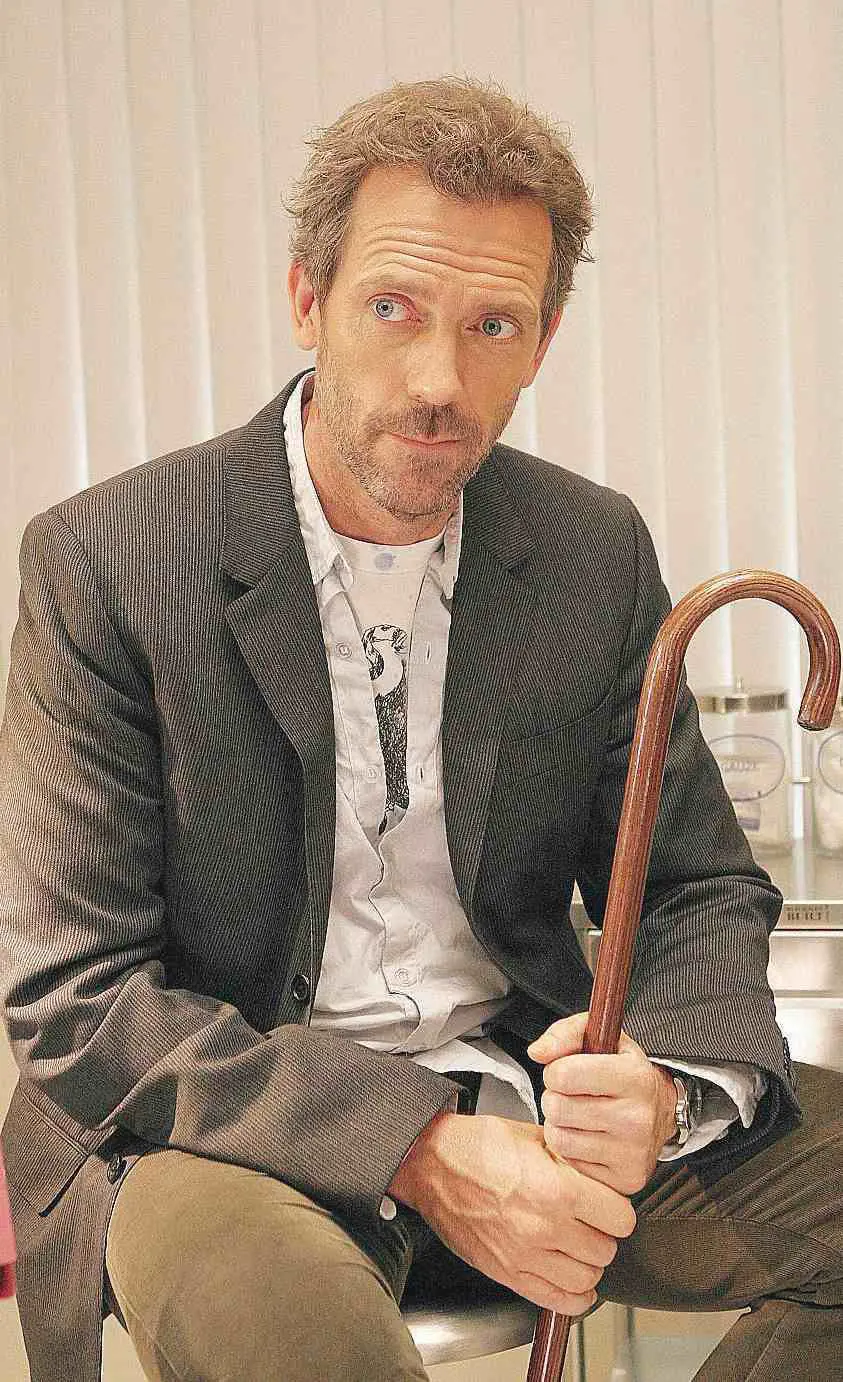
\includegraphics[height=3.5cm,keepaspectratio]{Dr-House.png}
				{\tiny\\LISP Dr. House\\\textbf{Sistema MYCIN (1972)}\\\vspace*{-4pt}\textit{\textcopyright ilGiornale.it}}
			\end{figure}
		\end{minipage}
		\hfill
		\begin{minipage}[b]{0.45\textwidth}
			\centering
			\begin{figure}[ht]
				\includegraphics[height=3.5cm,keepaspectratio]{XSEL-XCON-no-bg-explained.png}
				{\tiny\\\textbf{Sistema R1/XCON (1978)}\\\vspace*{-4pt}\textit{\textcopyright DOI:10.1145/62065.62067}}
			\end{figure}
		\end{minipage}
		\begin{center}
			\hyperlink{subsec:appendix-expert-systems}{\color{venis-faithful-yellow}\faExternalLinkSquare\ Maggiori informazioni}
		\end{center}		
	\end{minipage}
	}
	}
\end{frame}
%
\subsection{Rinascita della AI}
\label{subsec:ai_rise}
%
\begin{frame}[t,fragile] \frametitle{Cronistoria della AI}
	\framesubtitle{1975-2000: \ldots di nuovo alle stelle}
	\vspace*{-15pt}
	\begin{figure}[ht]
        \centering
        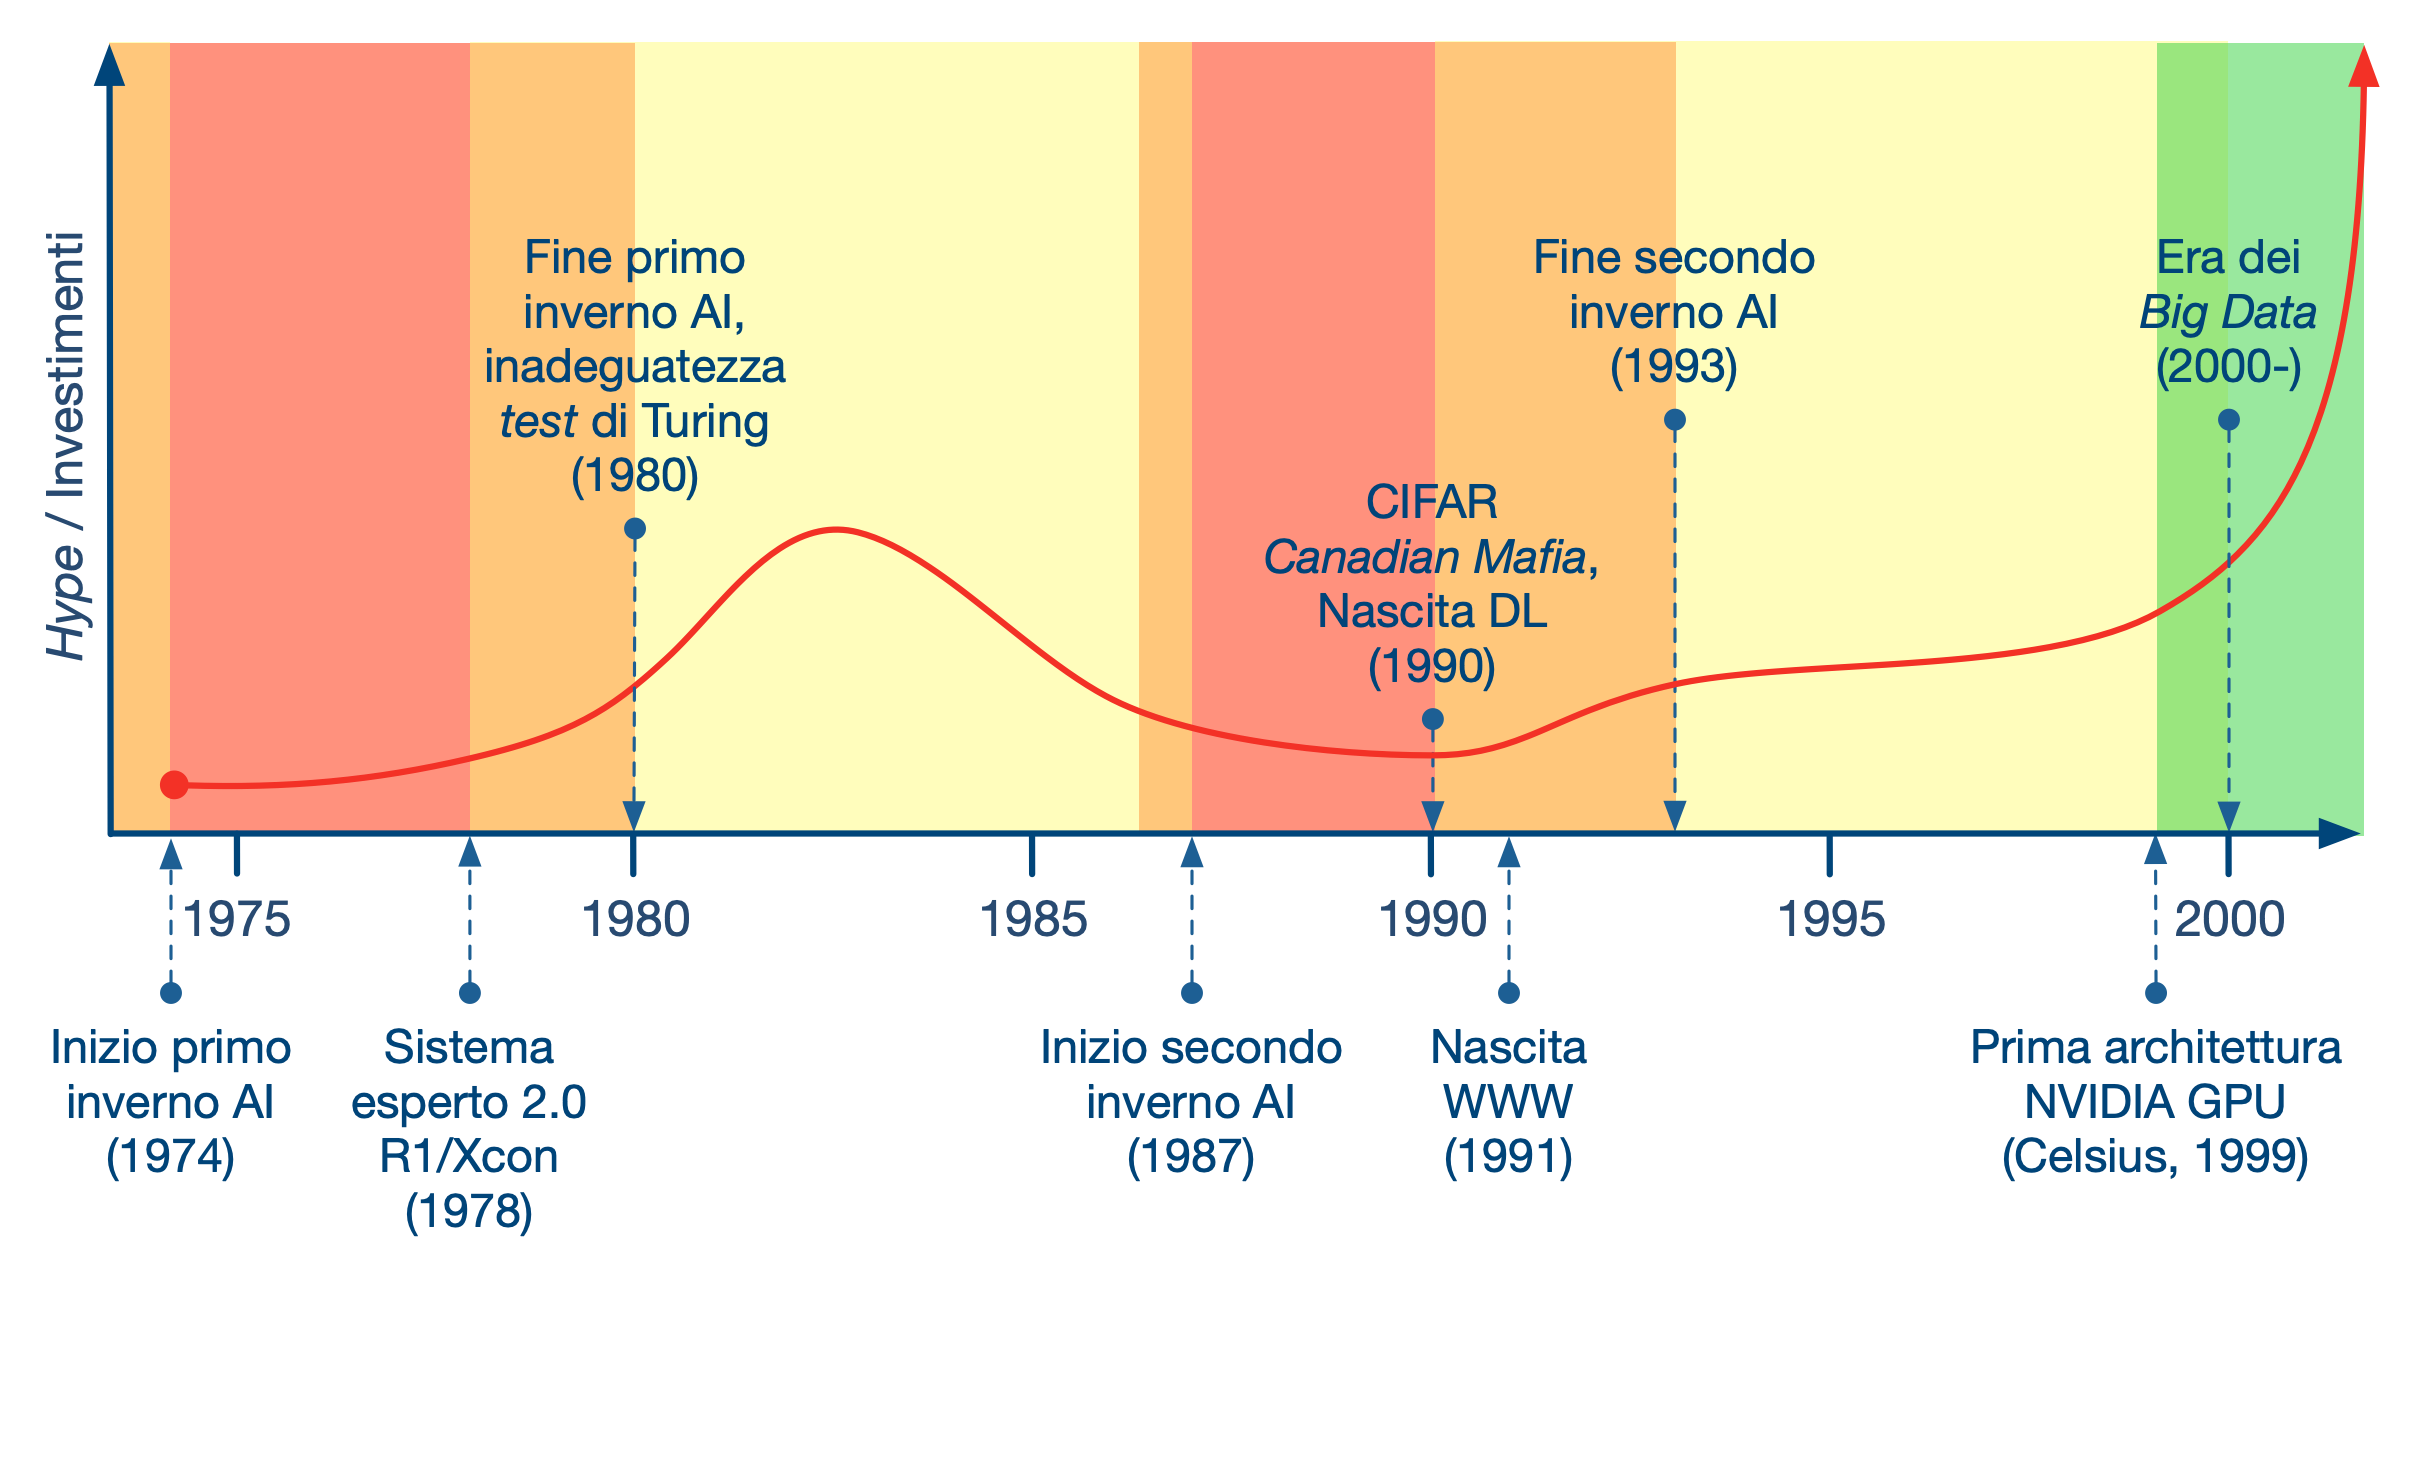
\includegraphics[width=\textwidth]{AI-rollercoaster-2.png}
    \end{figure}
	\begin{flushright}
    	\vspace*{-10pt}
        {\tiny\textit{\textcopyright Simone Scannapieco. I valori delle ordinate sono puramente indicativi.}}
	\end{flushright}
\end{frame}
%
\begin{frame}[t,fragile] \frametitle{Cronistoria della AI}
	\framesubtitle{1975-2000: fattori di ripresa}
	\vspace*{-.5cm}
	{\small
	\begin{itemize}[leftmargin=10pt,align=right]
		\item[\alert{\faArrowCircleRight}] \alert{Nascita del \textit{Deep Learning} (DL):} unità neuronali che collaborano in strutture ``profonde''
	\end{itemize}
	\only<1|handout:0>{
		\begin{minipage}[t]{\textwidth}
			\begin{figure}[ht]
				\centering
				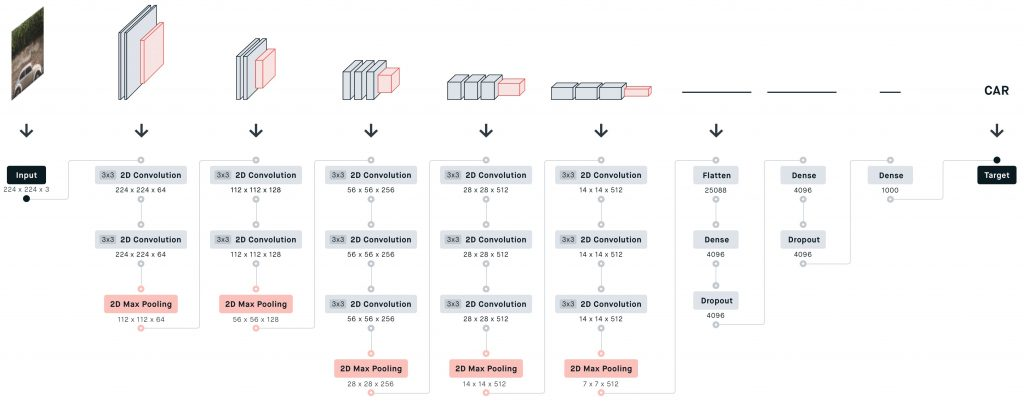
\includegraphics[width=.45\textwidth]{vgg-16-image-no-bg.png}
				{\tiny\\Architettura VGG-16\\\textit{\textcopyright LinkedIn}\\\vspace*{-4pt}\href{https://poloclub.github.io/cnn-explainer/}{\faExternalLinkSquare\ CNN Explainer}}
			\end{figure}
		\end{minipage}
		\vfill
		\begin{minipage}[t]{\textwidth}
			\begin{minipage}[b]{0.33\textwidth}
				\centering
				\begin{figure}[ht]
					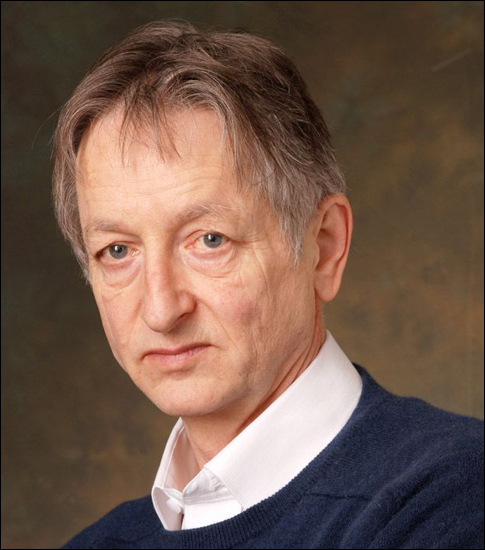
\includegraphics[width=.6\textwidth]{Geoffrey-Hinton.jpeg}
					{\tiny\\Geoffrey Hinton\\\vspace*{-4pt}\textit{\textcopyright acm.org}}
				\end{figure}
			\end{minipage}
			\begin{minipage}[b]{0.33\textwidth}
				\centering
				\begin{figure}[ht]
					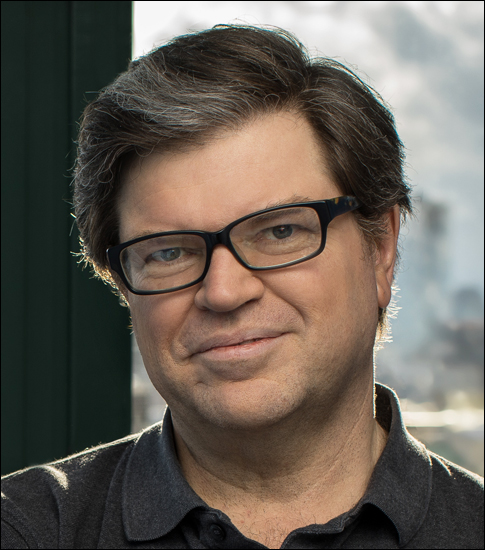
\includegraphics[width=.6\textwidth]{Yann-LeCun.jpeg}
					{\tiny\\Yann LeCun\\\vspace*{-4pt}\textit{\textcopyright acm.org}}
				\end{figure}
			\end{minipage}
			\begin{minipage}[b]{0.33\textwidth}
				\centering
				\begin{figure}[ht]
					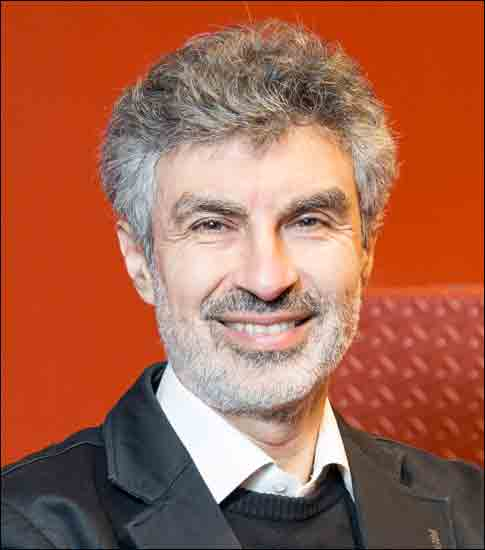
\includegraphics[width=.6\textwidth]{Yoshua-Bengio.jpeg}
					{\tiny\\Yoshua Bengio\\\vspace*{-4pt}\textit{\textcopyright acm.org}}
				\end{figure}
			\end{minipage}
		\end{minipage}
	}
	\only<2|handout:1>{
		\begin{minipage}[t]{\textwidth}
			\begin{figure}[ht]
				\centering
				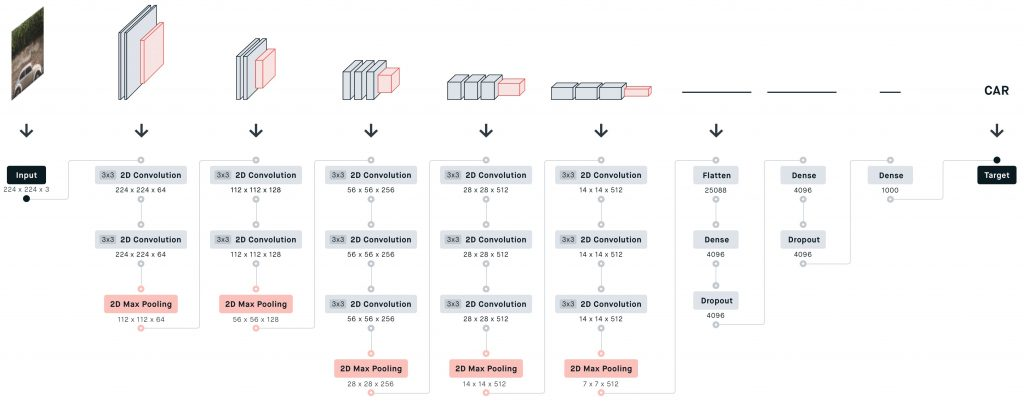
\includegraphics[width=.45\textwidth]{vgg-16-image-no-bg.png}
				{\tiny\\Architettura VGG-16\\\textit{\textcopyright LinkedIn}\\\vspace*{-4pt}\href{https://poloclub.github.io/cnn-explainer/}{\faExternalLinkSquare\ CNN Explainer}}
			\end{figure}
		\end{minipage}
		\vfill
		{\scriptsize
		\begin{minipage}[t]{\textwidth}
			\begin{minipage}[t]{.4\textwidth}
				\begin{itemize}[leftmargin=10pt,align=right]
					\item[\alert{\faArrowCircleRight}] Modello\\
					\begin{minipage}[t]{\textwidth}
						\renewcommand{\epigraphsize}{\scriptsize}
						\setlength{\afterepigraphskip}{0pt}
						\setlength{\beforeepigraphskip}{5pt}
						\setlength{\epigraphwidth}{0.9\textwidth}
						\epigraph{\textit{[\ldots] del modo in cui opera il sistema nervoso. Le unità di base sono costituite dai neuroni, in genere organizzati in strati [\ldots]}}{IBM (\href{https://www.ibm.com/docs/it/spss-modeler/18.5.0?topic=networks-neural-model}{Fonte}), 2004}
					\end{minipage}
				\end{itemize}
			\end{minipage}
			\hfill
			\begin{minipage}[t]{.5\textwidth}
				\begin{itemize}[leftmargin=10pt,align=right]
					\item[\alert{\faArrowCircleRight}] Architettura
					\begin{itemize}[leftmargin=20pt,align=right]
						\item[\alert{\faArrowCircleRight}] Dimensione dell'\emph{input}/\emph{output}
			 			\item[\alert{\faArrowCircleRight}] Numero di strati (pi\'{u} strati implica apprendimento pi\'{u} complesso)
						\item[\alert{\faArrowCircleRight}] Funzione di attivazione di ciascun strato
						\item[\alert{\faArrowCircleRight}] Numero di neuroni per strato
						\item[\alert{\faArrowCircleRight}] Funzione costo da minimizzare
					\end{itemize}
				\end{itemize}
			\end{minipage}
			\begin{center}
				\hyperlink{subsec:cnn}{\color{venis-faithful-yellow}\faExternalLinkSquare\ Maggiori informazioni}
			\end{center}		
		\end{minipage}
		}
	}
	\only<3|handout:0>{
		\begin{figure}[ht]
        	\centering
        	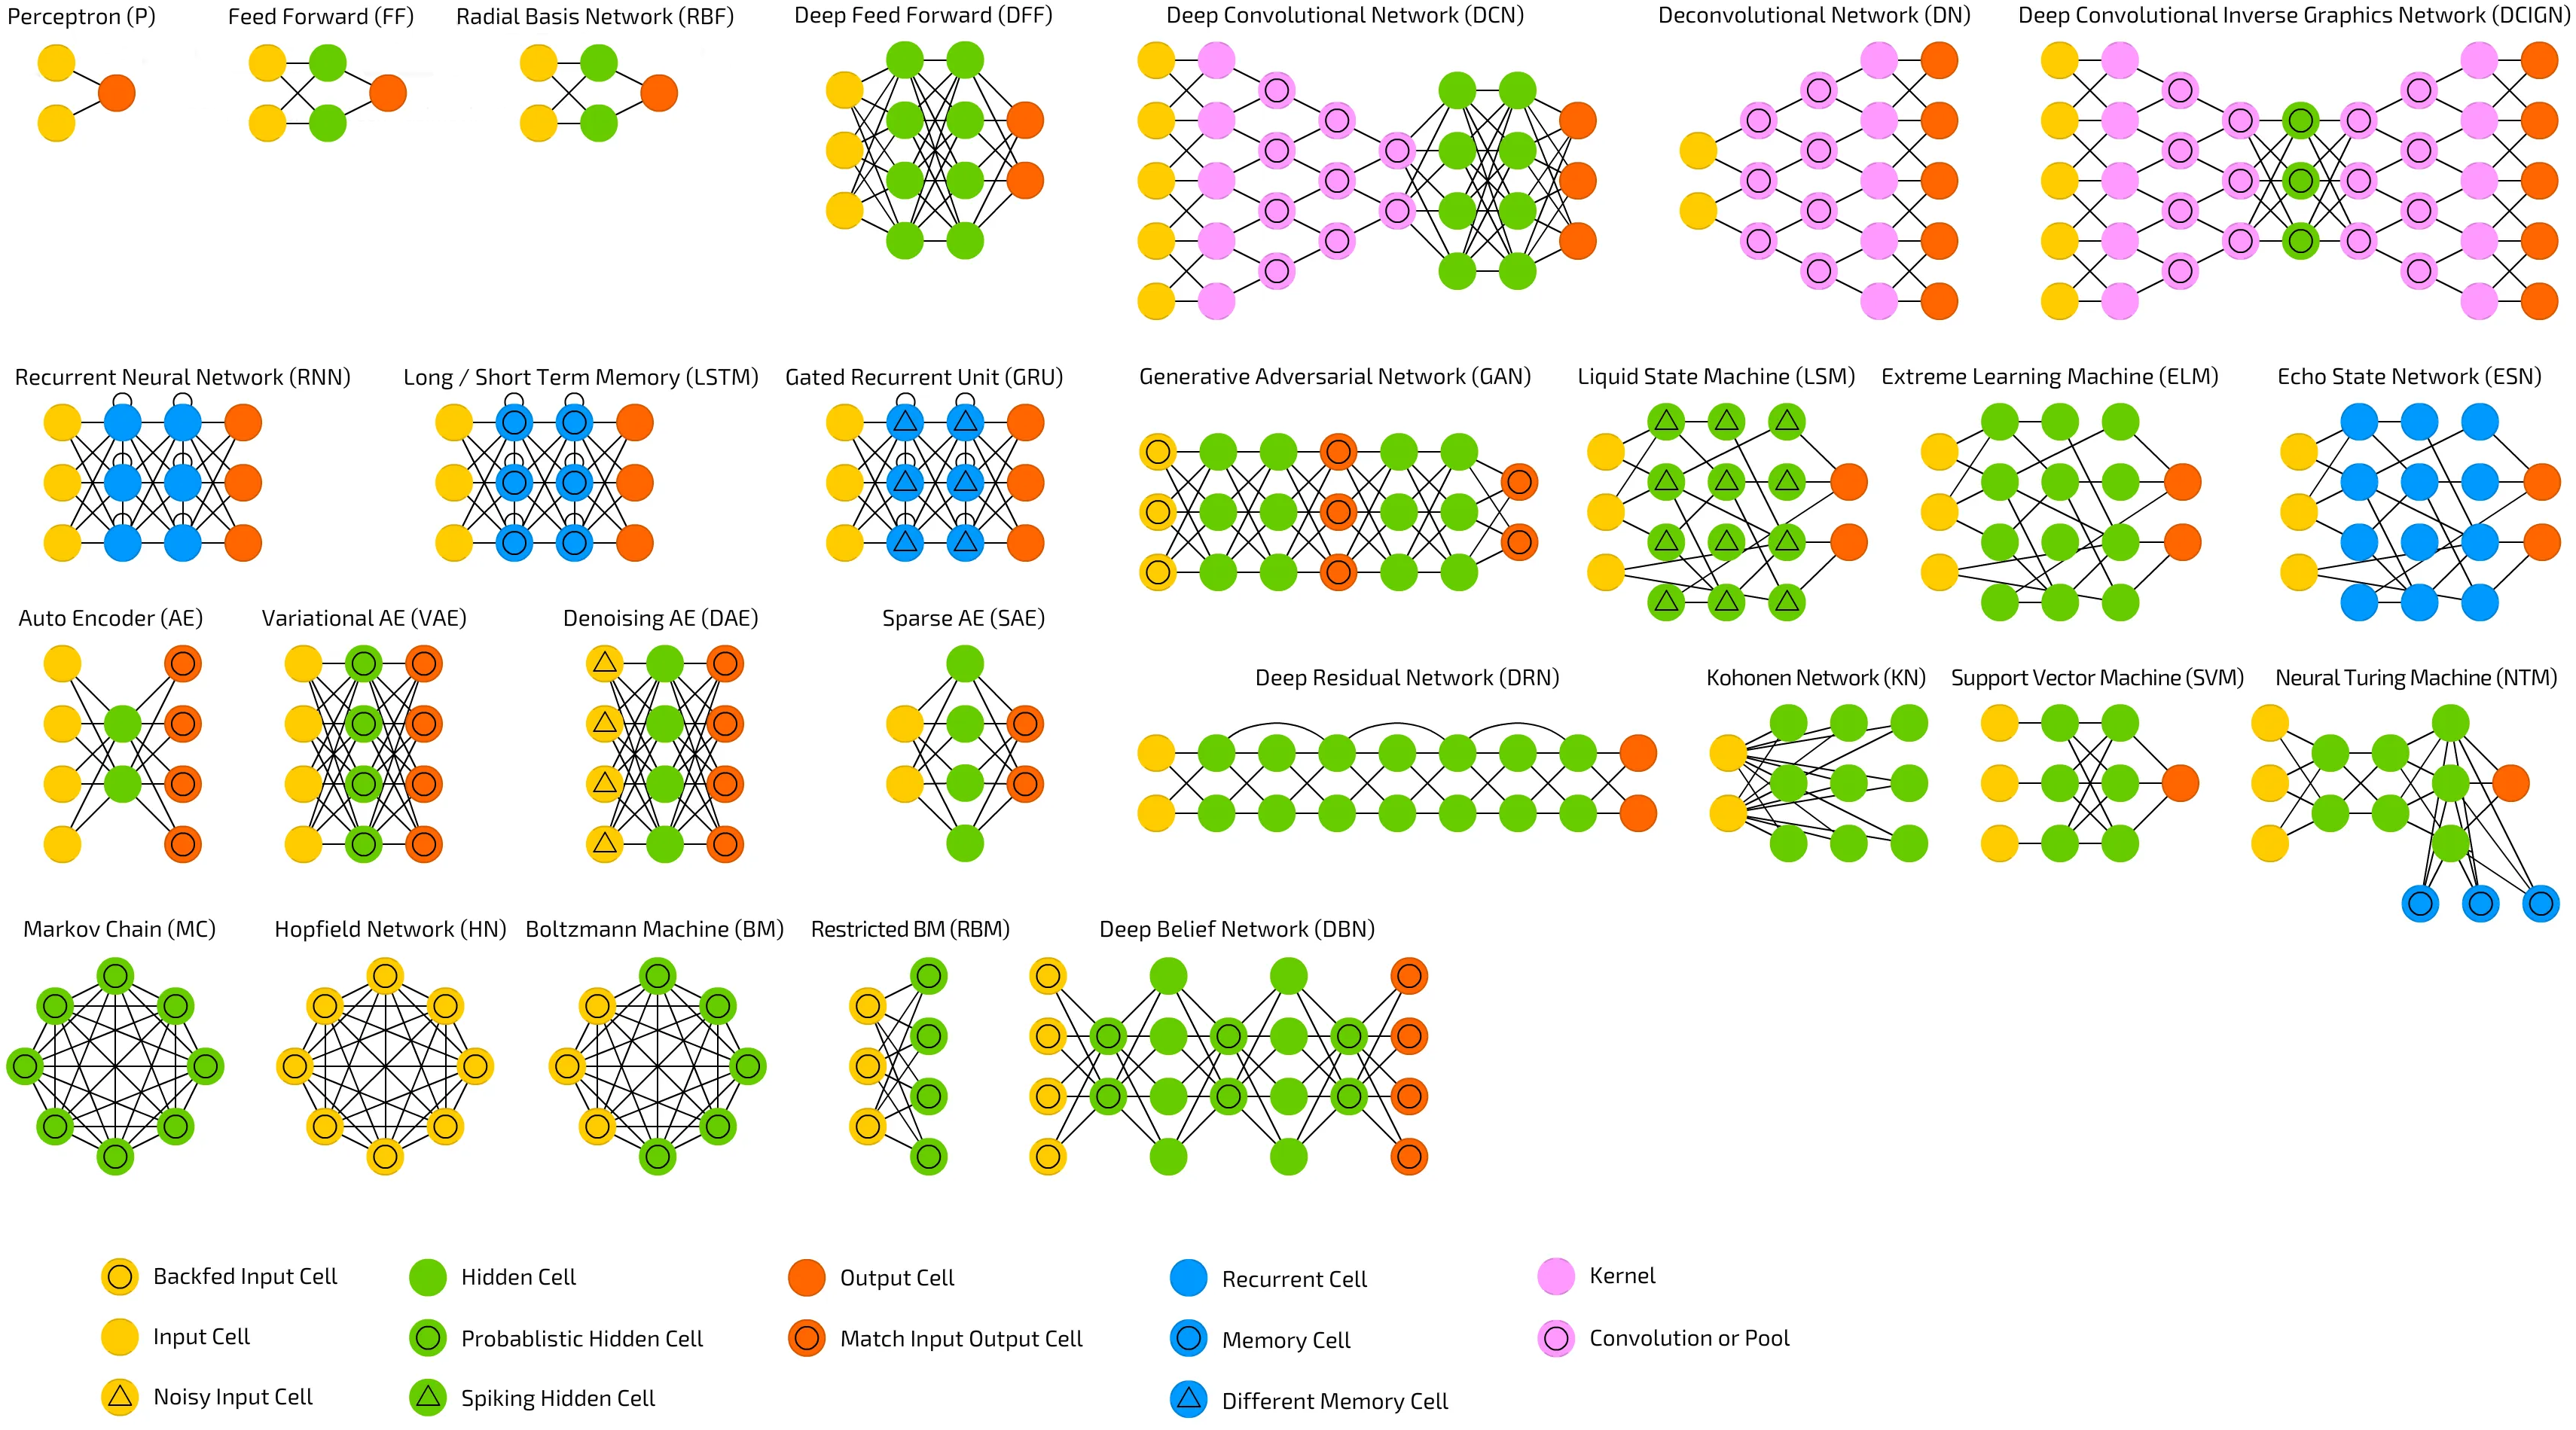
\includegraphics[width=.8\textwidth]{neural-networks-chart-alpha-rearranged.png}
    	\end{figure}
		\begin{flushright}
    		\vspace*{-10pt}
        	{\tiny\textit{\textcopyright Fjodor van Veen, Andrew Tch, Medium}}
		\end{flushright}
	}
	\only<4|handout:2>{
		\begin{figure}[ht]
        	\centering
        	\includegraphics[width=.8\textwidth]{neural-networks-chart-alpha-rearranged-highlighted.png}
    	\end{figure}
		\begin{flushright}
    		\vspace*{-10pt}
        	{\tiny\textit{\textcopyright Fjodor van Veen, Andrew Tch, Medium}}
		\end{flushright}
	}
}
\end{frame}
%
\begin{frame}[t,fragile] \frametitle{Cronistoria della AI}
	\framesubtitle{1975-2000: fattori di ripresa}
	\vspace*{-.5cm}
	{\small
		\begin{itemize}[leftmargin=10pt,align=right]
			\onslide<1->\item[\alert{\faArrowCircleRight}] \alert{Maturità tecnologica:} algoritmi di addestramento e \textit{hardware} sempre più efficienti
		\end{itemize}
		\vfill
		\begin{minipage}[t]{\textwidth}
			\begin{minipage}[b]{0.45\textwidth}
				\centering
				\begin{figure}[ht]
					\centering
					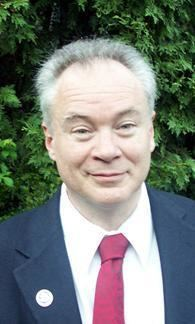
\includegraphics[height=3.5cm,keepaspectratio]{Paul-Werbos.jpg}
					{\tiny\\Paul Werbos\\\textbf{Algoritmo di retro-propagazione (Springer, 1982)}\\\vspace*{-4pt}\textit{\textcopyright Alchetron.com}}
				\end{figure}
			\end{minipage}
			\hfill
			\begin{minipage}[b]{0.45\textwidth}
				\centering
				\begin{figure}[ht]
					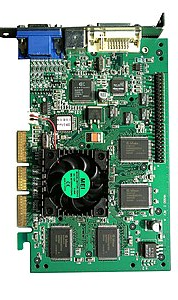
\includegraphics[height=3.5cm,keepaspectratio]{VisionTek_GeForce_256_rotated.png}
					{\tiny\\Architetture GPU dedicate alla supercomputazione\\\textbf{NVIDIA GeForce 256 Celsius (1999)}\\\vspace*{-4pt}\textit{\textcopyright Wikimedia Creative Commons}}
				\end{figure}
			\end{minipage}
		\end{minipage}
	}
\end{frame}
%
\begin{frame}[t,fragile] \frametitle{Cronistoria della AI}
	\framesubtitle{1975-2000: fattori di ripresa}
	\vspace*{-.5cm}
	{\small
		\begin{itemize}[leftmargin=10pt,align=right]
			\onslide<1->\item[\alert{\faArrowCircleRight}] \alert{Nascita del WWW:} apre le porte alla \alert{democratizzazione dell'informazione} e al \textit{boom} del fenomeno \alert{\textit{big data}}
		\end{itemize}
		\vspace*{.3cm}
		\only<1|handout:1>{
		\begin{center}
			\begin{minipage}[b]{.45\textwidth}
				\begin{figure}[ht]
					\centering
					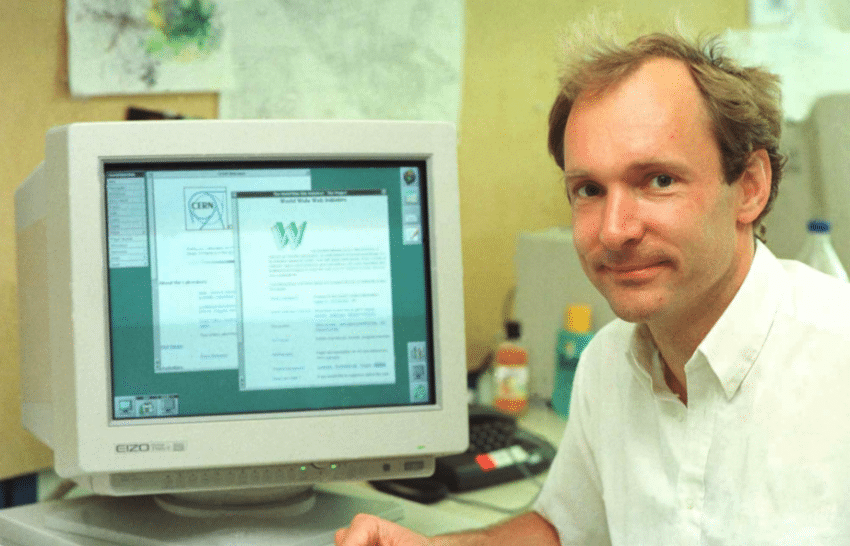
\includegraphics[width=\textwidth]{tim-berners-lee.png}
					{\tiny\\Tim Berners-Lee\\\textbf{Progetto WorldWideWeb - Nexus (1989-1991-1993)}\\\vspace*{-4pt}\textit{\textcopyright CERN}}
				\end{figure}
			\end{minipage}
			\\\vspace*{.3cm}
			\href{http://info.cern.ch}{\faExternalLinkSquare\ Per i nostalgici\ldots}
		\end{center}
		}
		\only<2|handout:0>{
		\begin{center}
			\begin{minipage}[b]{.6\textwidth}
				\begin{figure}[ht]
					\centering
					\includegraphics[width=\textwidth]{global-data-generated-annually-alpha.png}
				\end{figure}
				\begin{flushright}
                	\vspace*{-10pt}
                	{\tiny\textit{\textcopyright explodingtopics.com}}
            	\end{flushright}
			\end{minipage}
		\end{center}
		}
		\only<3|handout:2>{
		\begin{center}
			\begin{minipage}[b]{.6\textwidth}
				\begin{figure}[ht]
					\centering
					\includegraphics[width=\textwidth]{global-data-generated-annually-alpha-numbers.png}
				\end{figure}
				\begin{flushright}
                	\vspace*{-10pt}
                	{\tiny\textit{\textcopyright explodingtopics.com}}
            	\end{flushright}
			\end{minipage}
		\end{center}
		}
	}
\end{frame}
%
\section{Approfondimenti}
\label{sec:appendix}
%
\subsection{The Logic Theorist}
\label{subsec:logic-theorist}
%
\begin{frame}[t,fragile] \frametitle{Cronistoria della AI}
{\scriptsize
\onslide<1->
\framesubtitle{Primo programma di ricerca in AI}
\vspace*{-.5cm}
	\begin{minipage}[t]{\textwidth}
		\begin{figure}[ht]
			\centering
			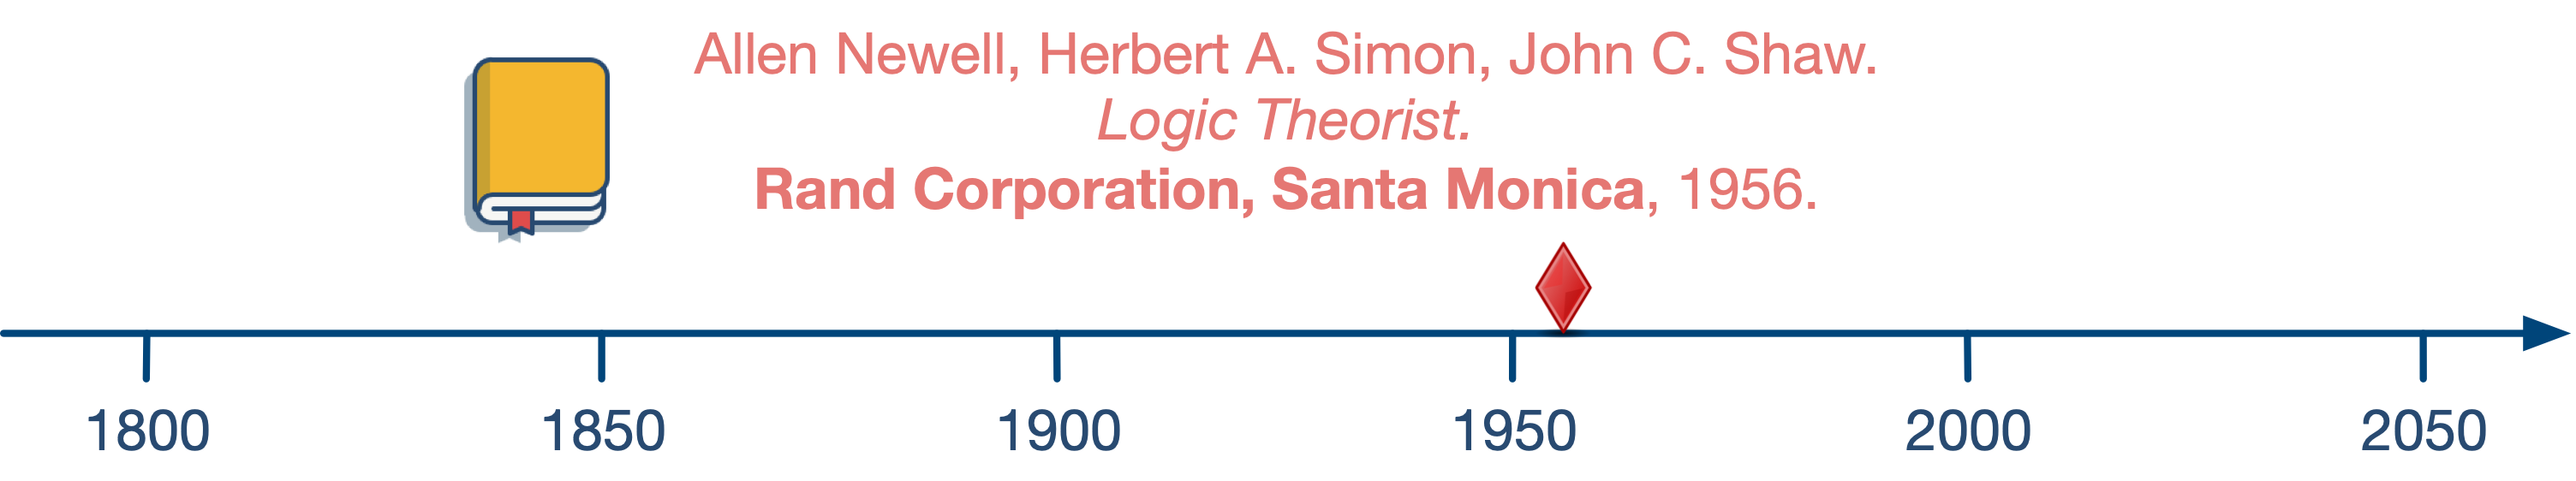
\includegraphics[width=\textwidth]{AI-timeline-1956-alt.png}
		\end{figure}
	\end{minipage}
	\\\vspace*{.3cm}
	\onslide<1->
	\begin{minipage}[b]{\textwidth}
		\begin{minipage}[b]{0.32\textwidth}
			\centering
			\begin{figure}[ht]
				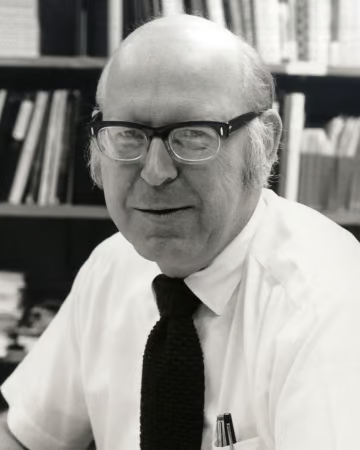
\includegraphics[width=.6\textwidth]{Allen-Newell.png}
				{\tiny\\Allen Newell\\\textit{\textcopyright On This Day}}
			\end{figure}
		\end{minipage}
		\begin{minipage}[b]{0.32\textwidth}
			\centering
			\begin{figure}[ht]
				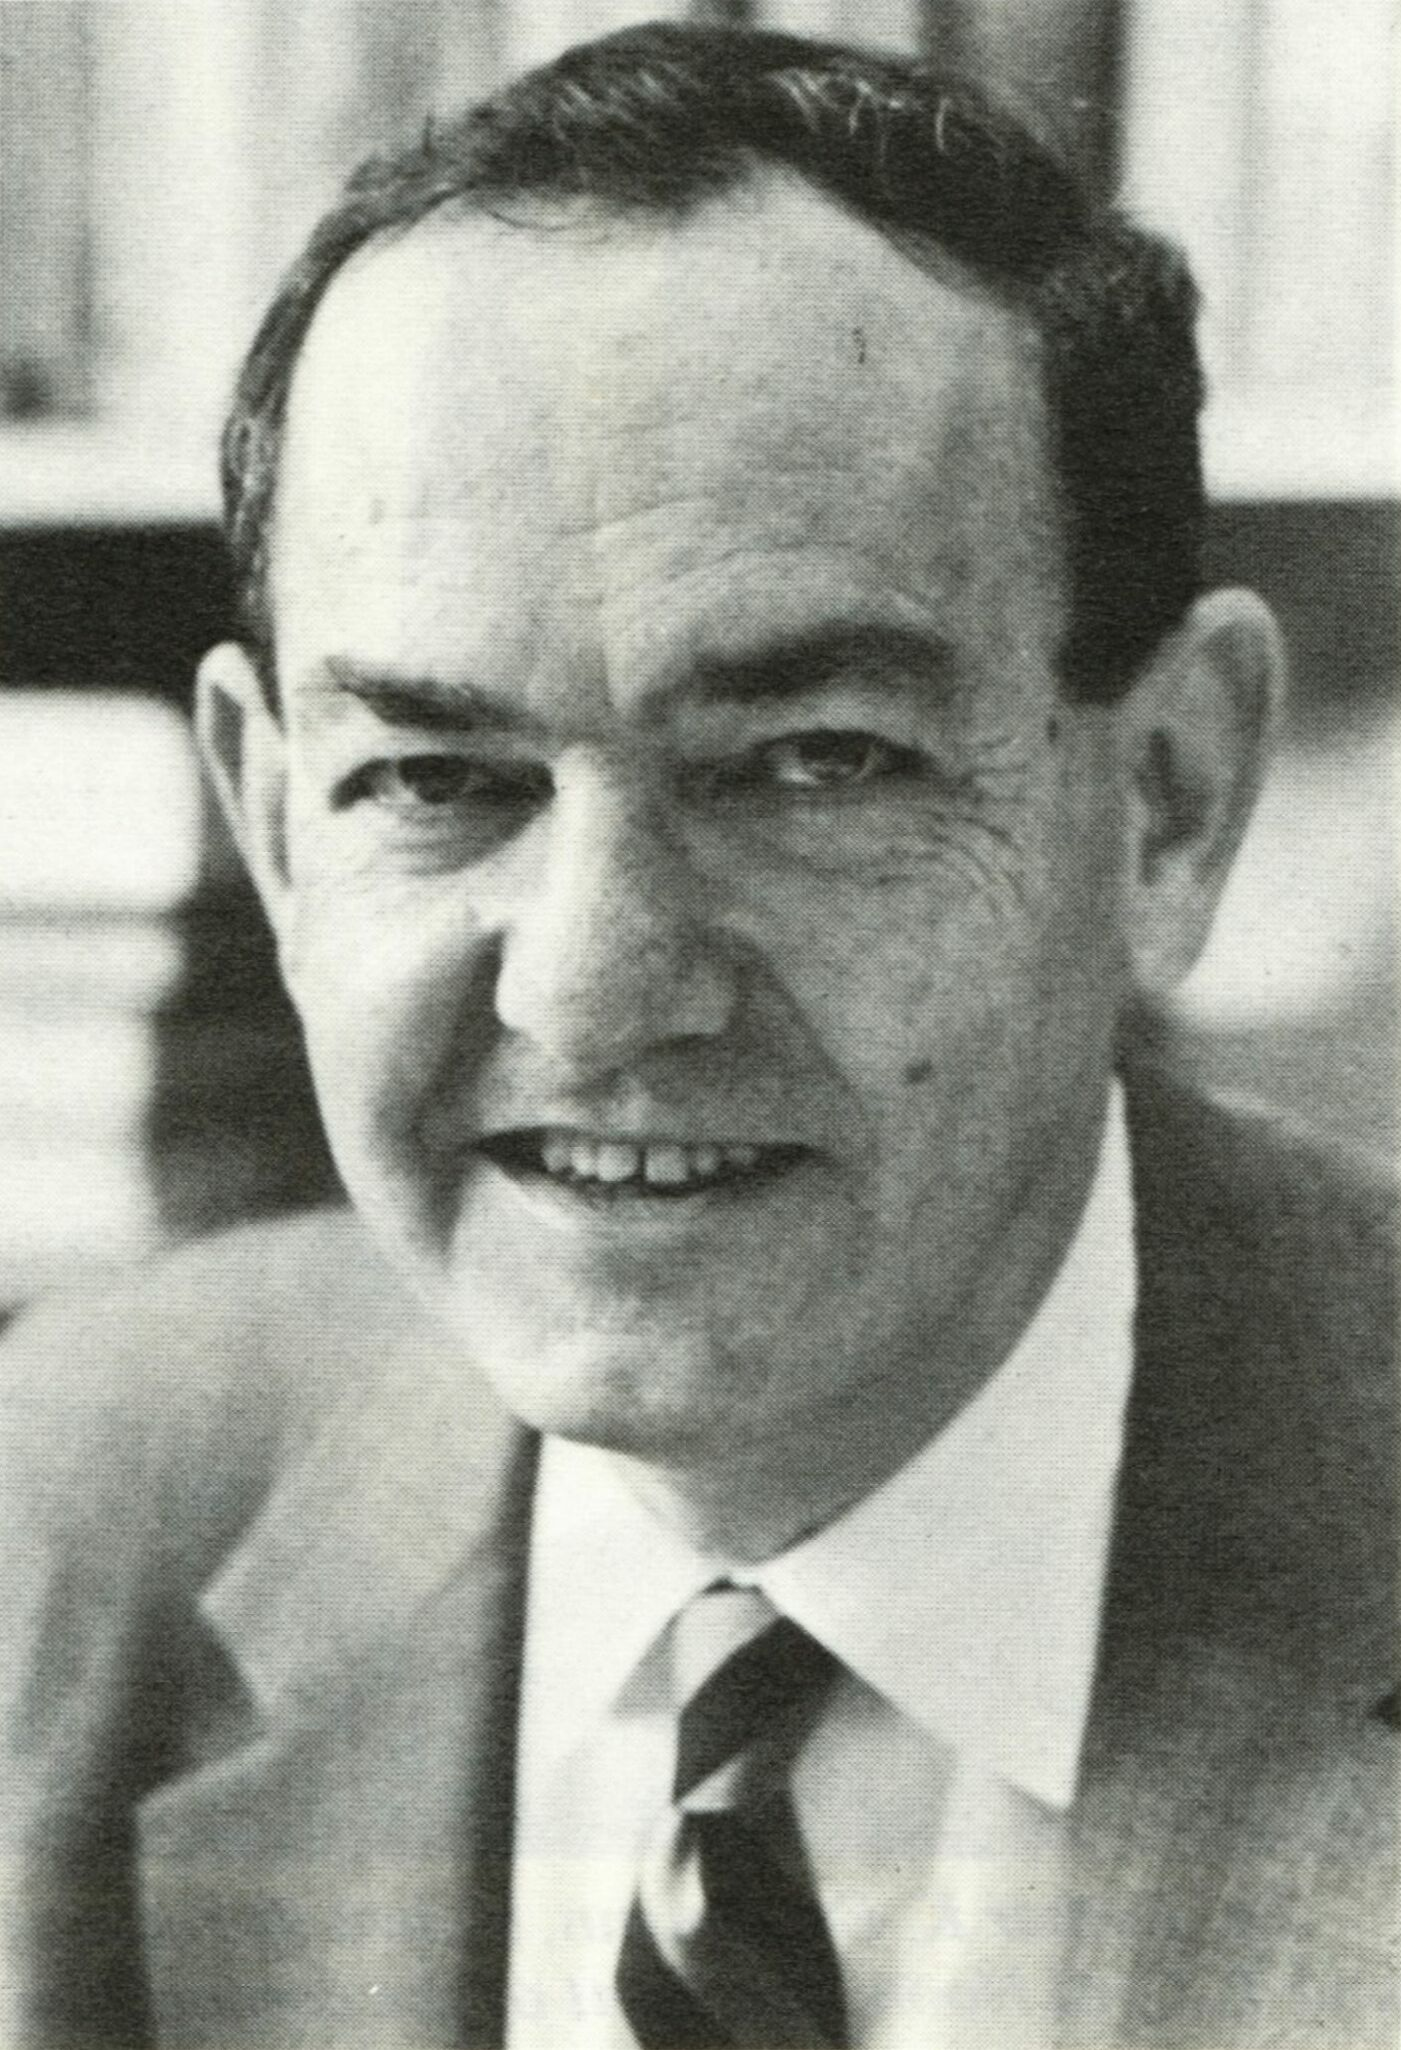
\includegraphics[width=.55\textwidth]{Herbert-Simon.jpg}
				{\tiny\\Herbert A. Simon\\\textit{\textcopyright Wikimedia Creative Commons}}
			\end{figure}
		\end{minipage}
		\begin{minipage}[b]{0.32\textwidth}
			\centering
			\begin{figure}[ht]
				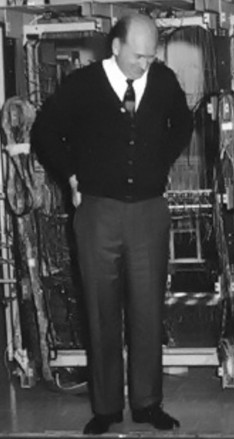
\includegraphics[width=.45\textwidth]{John-Shaw.jpg}
				{\tiny\\John C. Shaw\\\textit{\textcopyright Computer Timeline}}
			\end{figure}
		\end{minipage}
		\begin{center}
			\href{http://www.computer-timeline.com/timeline/logic-theorist-simon-newell-and-shaw/}{\faExternalLinkSquare\ Maggiori informazioni}
		\end{center}
	\end{minipage}
	%\begin{itemize}[leftmargin=10pt,align=right]
		%\onslide<2->\item[\alert{\faArrowCircleRight}] Nato \textit{per imitare le capacità di problem solving degli esseri umani}
		%\onslide<3->\item[\alert{\faArrowCircleRight}] In concomitanza con lo sviluppo dei primi linguaggi di programmazione dedicati (LISP)
	%\end{itemize}
}
\end{frame}
%
\subsection{Sistemi esperti}
\label{subsec:appendix-expert-systems}
%
\begin{frame}[t,fragile] \frametitle{Cronistoria della AI}
{\scriptsize
\onslide<1->
\framesubtitle{Prima resistenza al primo inverno della AI: i sistemi esperti}
\vspace*{-.5cm}
	\begin{minipage}[t]{\textwidth}
		\begin{figure}[ht]
			\centering
			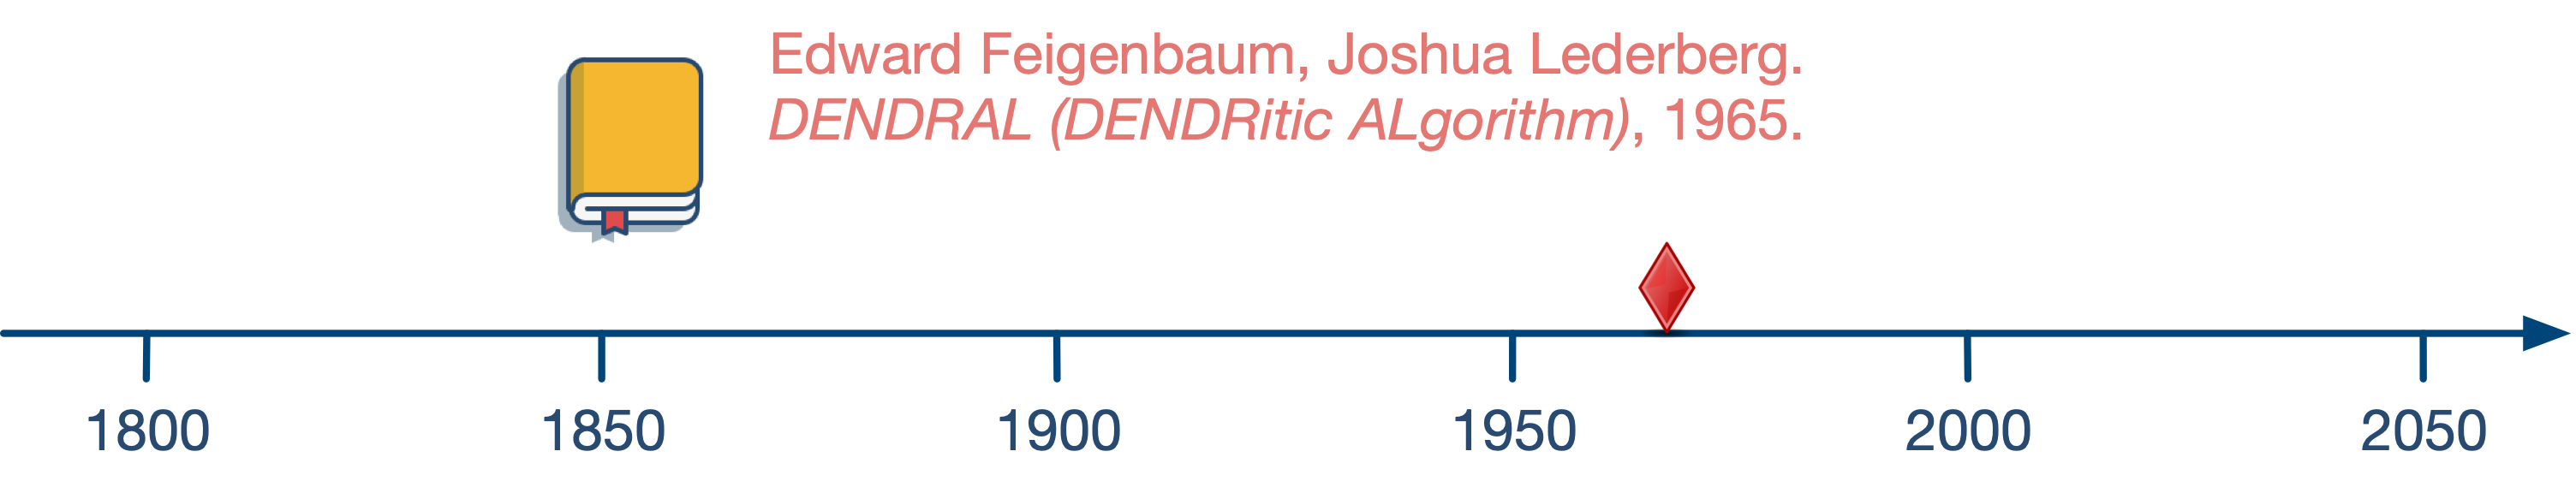
\includegraphics[width=\textwidth]{AI-timeline-1965-alt.png}
		\end{figure}
	\end{minipage}
	\\\vspace*{.3cm}
	\begin{minipage}[t]{\textwidth}
		\begin{minipage}[t]{0.6\textwidth}
			\begin{itemize}[leftmargin=10pt,align=right]
				\onslide<2->\item[\alert{\faArrowCircleRight}] \emph{Perceptron} di Rosenblatt come ``capro espiatorio'' dell'inverno AI
				\begin{itemize}[leftmargin=10pt,align=right]
					\item[\alert{\faArrowCircleRight}] Scarsa capacità di \alert{elaborazione} e \alert{memorizzazione} delle informazioni
				\end{itemize}
				\onslide<3->\item[\alert{\faArrowCircleRight}] \alert{Sistemi esperti} -- ES (o \alert{basati sulla conoscenza} -- KBS)
				\begin{itemize}[leftmargin=10pt,align=right]
					\item[\alert{\faArrowCircleRight}] Sistema informatico specializzato in un determinato campo o materia
					\item[\alert{\faArrowCircleRight}] Conoscenza come base di dati strutturate + regole di ragionamento
				\end{itemize}
				\onslide<4->\item[\alert{\faArrowCircleRight}] DENDRAL specializzato in ambito \alert{chimico} (riconoscimento di molecole organiche sconosciute)
			\end{itemize}
		\end{minipage}
		%
		\onslide<1->
		\begin{minipage}[t]{0.4\textwidth}
			\centering
			\begin{figure}[ht]
				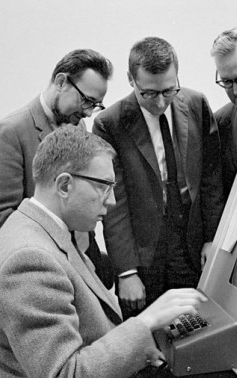
\includegraphics[width=.55\textwidth]{Edward-Feigenbaum-crop.png}
				{\tiny\\Edward Feigenbaum\\\textit{\textcopyright Klondike.ai}}
			\end{figure}
		\end{minipage}
	\end{minipage}
}
\end{frame}
%
\begin{frame}[t,fragile] \frametitle{Cronistoria della AI}
{\scriptsize
\onslide<1->
\framesubtitle{Prima resistenza al primo inverno della AI: i Sistemi Esperti}
\vspace*{-.5cm}
	\begin{minipage}[t]{\textwidth}
		\begin{figure}[ht]
			\centering
			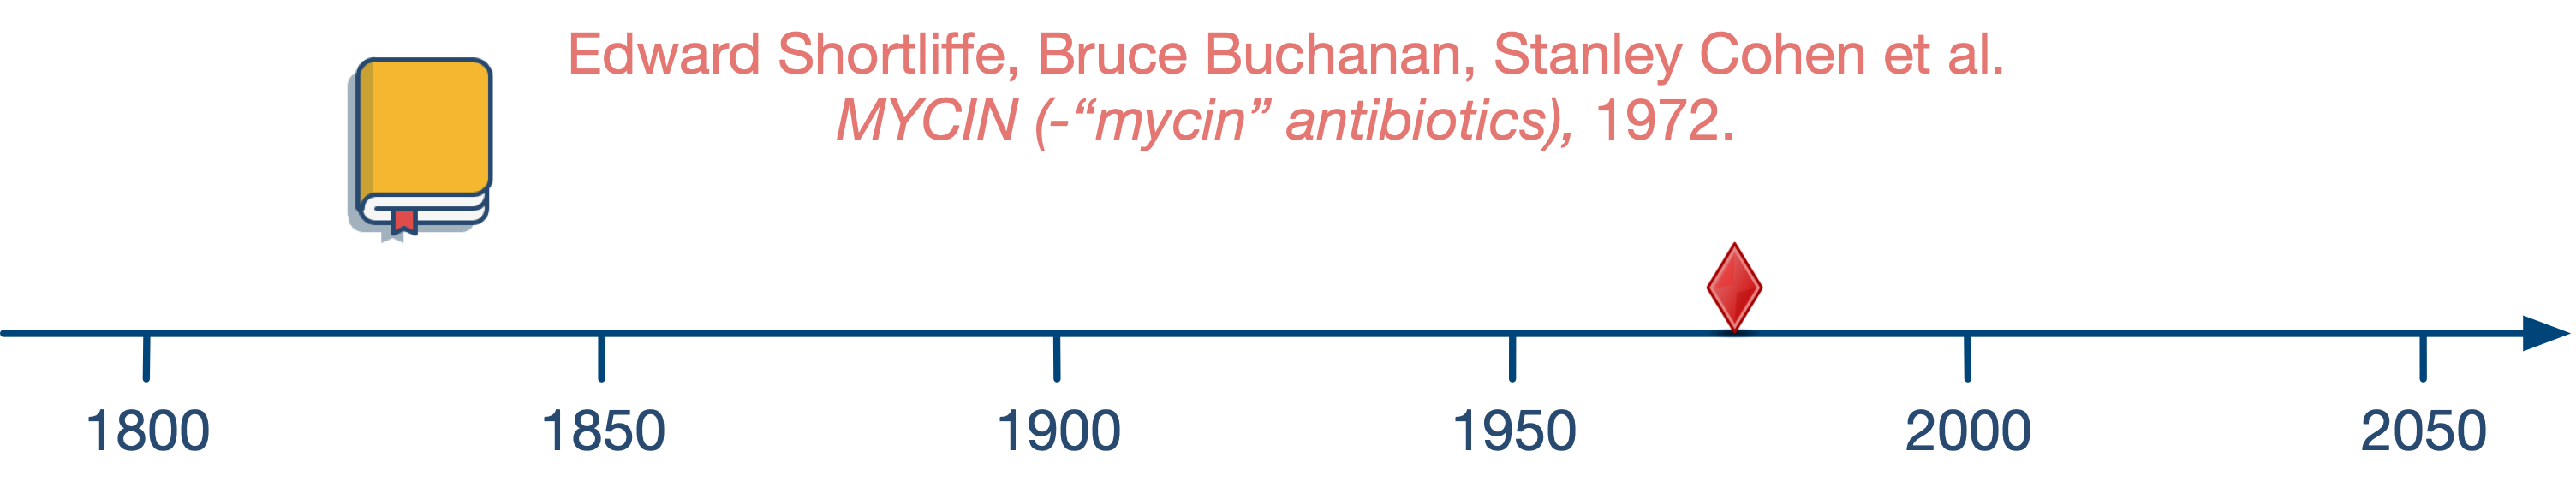
\includegraphics[width=\textwidth]{AI-timeline-1972-alt.png}
		\end{figure}
	\end{minipage}
	\\\vspace*{.3cm}
	\begin{minipage}[t]{\textwidth}
		\begin{minipage}[t]{0.6\textwidth}
			\begin{itemize}[leftmargin=10pt,align=right]
				\onslide<2->\item[\alert{\faArrowCircleRight}] Sistema istruito in ambito \alert{medico}
				\begin{itemize}[leftmargin=10pt,align=right]
					\onslide<3->\item[\alert{\faArrowCircleRight}] Identificazione di batteri nel sangue
					\item[\alert{\faArrowCircleRight}] Assistenza ai medici nella diagnosi delle malattie infettive
					\item[\alert{\faArrowCircleRight}] Una implementazione LISP di ``Dr. House'' che ragionava in algebra booleana e con logica del primo ordine ($\textrm{cause} \rightarrow \textrm{effetto}$)$\ldots$
					\onslide<4->\item[\alert{\faArrowCircleRight}] $\ldots$ ma sicuramente \emph{less miserable} (cit.)
					\onslide<4->\item[\alert{\faExclamationTriangle}] Se non avete visto la serie, \textbf{\alert{pentitevi} e \alert{rimediate}}
				\end{itemize}
			\end{itemize}
		\end{minipage}
		%
		\onslide<1->
		\begin{minipage}[t]{0.4\textwidth}
			\centering
			\begin{figure}[ht]
				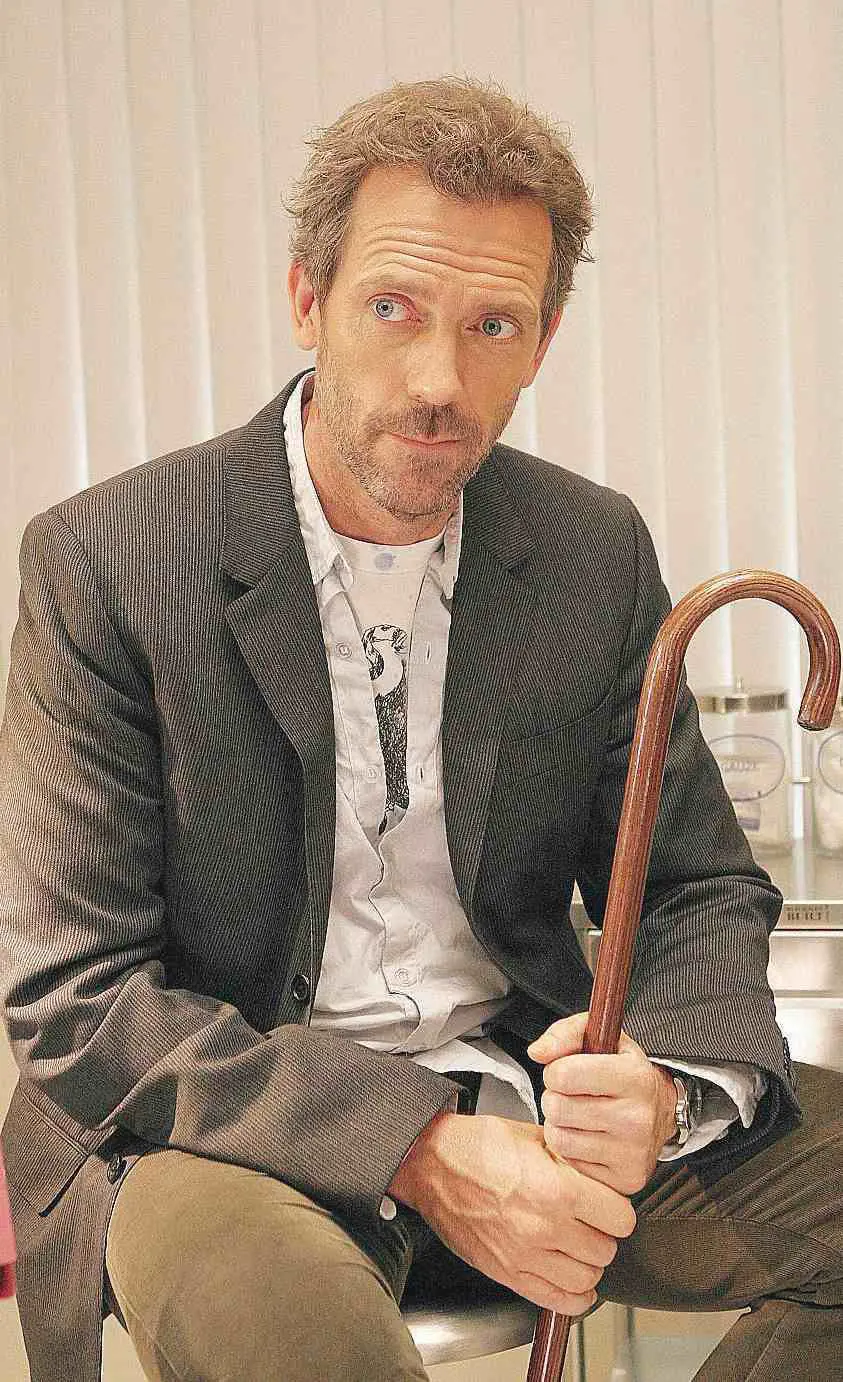
\includegraphics[width=.5\textwidth]{Dr-House.png}
				{\tiny\\Dr. House\\\textit{\textcopyright ilGiornale.it}}
			\end{figure}
		\end{minipage}
	\end{minipage}
}
\end{frame}
%
\begin{frame}[t,fragile] \frametitle{Cronistoria della AI}
{\scriptsize
\onslide<1->
\framesubtitle{Sistemi esperti 2.0}
\vspace*{-.5cm}
	\begin{minipage}[t]{\textwidth}
		\begin{figure}[ht]
			\centering
			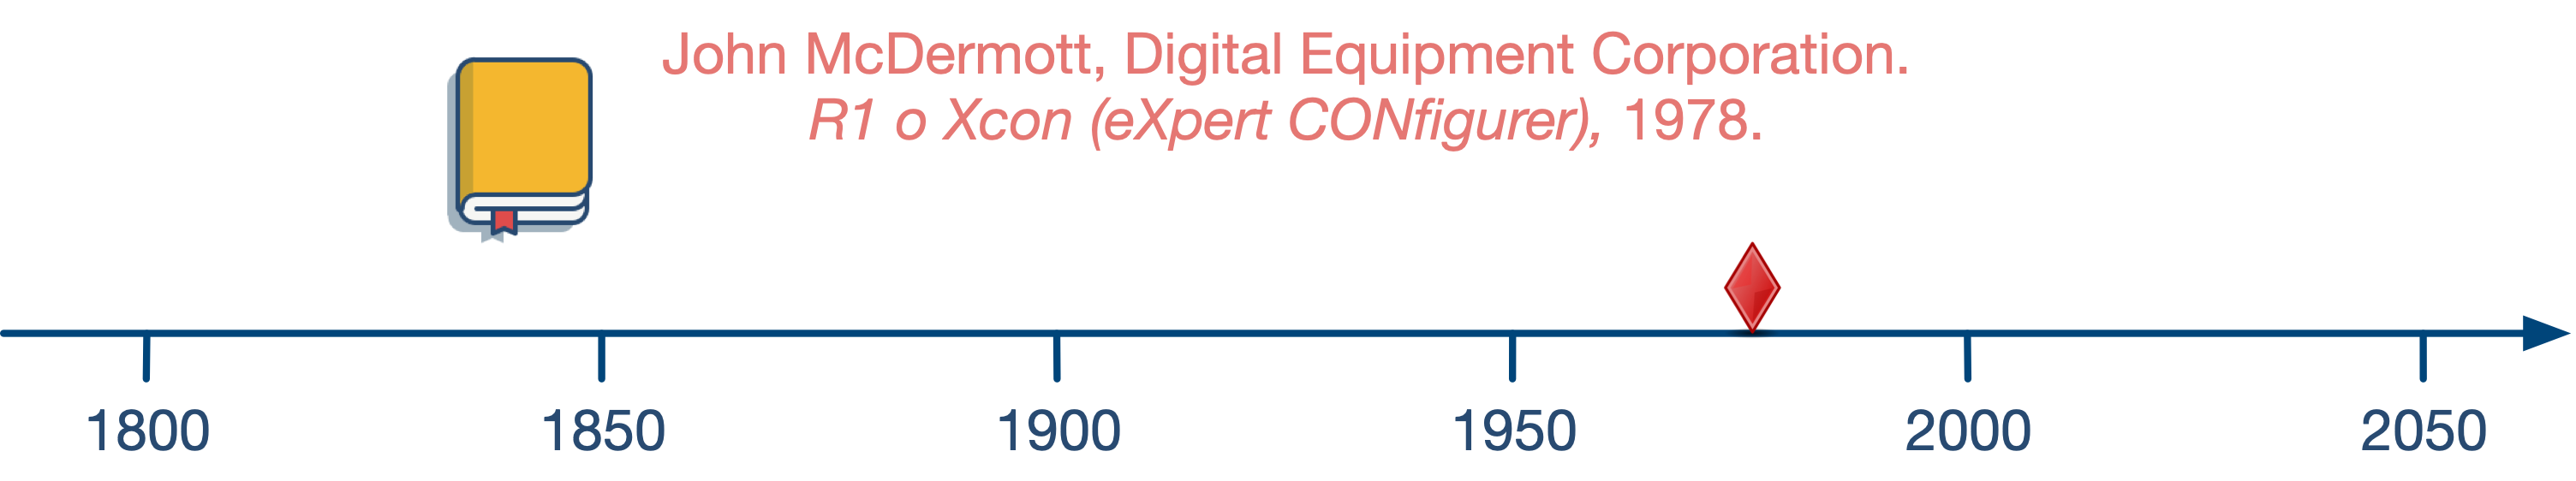
\includegraphics[width=\textwidth]{AI-timeline-1978-alt.png}
		\end{figure}
	\end{minipage}
	\\\vspace*{.3cm}
	\begin{minipage}[t]{\textwidth}
		\begin{minipage}[t]{0.6\textwidth}
			\begin{itemize}[leftmargin=10pt,align=right]
				\onslide<2->\item[\alert{\faArrowCircleRight}] Sistema utilizzato in ambito \alert{industriale/commerciale}
				\begin{itemize}[leftmargin=10pt,align=right]
					\onslide<3->\item[\alert{\faArrowCircleRight}] Configuratore intelligente di calcolatori
					\item[\alert{\faArrowCircleRight}] Verificatore di completezza degli ordini e ottimizzatore delle disposizioni
					\item[\alert{\faArrowCircleRight}] Risparmio stimato: 40m\$ in 4 anni
				\end{itemize}
				\onslide<4->\item[\alert{\faArrowCircleRight}] Spinta per nuovi fondi per la ricerca AI (Giappone, USA, GB, Europa)$\ldots$
				\onslide<5->\item[\alert{\faArrowCircleRight}]$\ldots$ ma vincoli operativi insiti
				\begin{itemize}[leftmargin=10pt,align=right]
					\item[\alert{\faArrowCircleRight}] Codifica KBs e regole estremamente difficile
				\end{itemize}
				\item[\alert{\faArrowCircleRight}] Risultato: \alert{secondo inverno della AI}
			\end{itemize}
		\end{minipage}
		%
		\onslide<1->
		\begin{minipage}[t]{0.4\textwidth}
			\centering
			\begin{figure}[ht]
				\includegraphics[width=\textwidth]{XSEL-XCON-no-bg-explained.png}
				{\tiny\\\textbf{Sistema R1/XCON (1978)}\\\textit{\textcopyright DOI:10.1145/62065.62067}}
			\end{figure}
		\end{minipage}
		\onslide<5->
		\begin{center}
			\hyperlink{subsec:ai_fall}{\color{venis-faithful-yellow}\faExternalLinkSquare\ Indietro}
		\end{center}
	\end{minipage}
}
\end{frame}
%
\subsection{Critihce a Turing}
\label{subsec:searle}
%
\begin{frame}[t,fragile] \frametitle{Cronistoria della AI}
{\scriptsize
\onslide<1->
\framesubtitle{Intelligenza sintetica stupida}
\vspace*{-.5cm}
	\begin{minipage}[t]{\textwidth}
		\begin{figure}[ht]
			\centering
			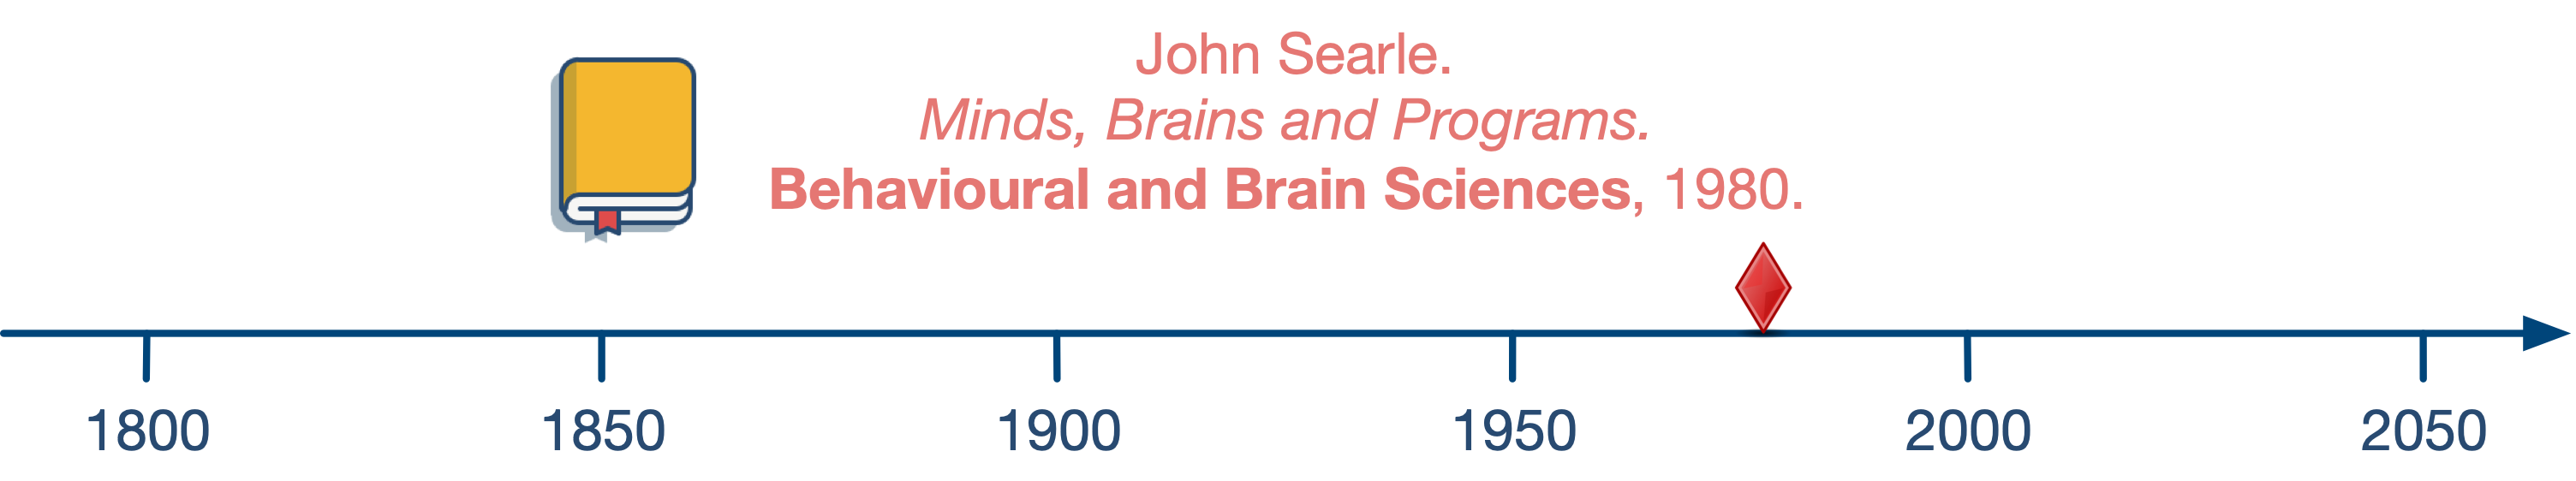
\includegraphics[width=\textwidth]{AI-timeline-1980-alt.png}
		\end{figure}
	\end{minipage}
	\\\vspace*{.3cm}
	\begin{minipage}[t]{\textwidth}
		\begin{minipage}[t]{0.6\textwidth}
			\begin{itemize}[leftmargin=10pt,align=right]
				\onslide<2->\item[\alert{\faArrowCircleRight}] Accanito sostenitore dell'inadeguatezza del \emph{test} di Turing
				\onslide<3->\item[\alert{\faArrowCircleRight}] Esercizio di pensiero (\alert{argomento delle stanze cinesi})
				\onslide<4->\begin{itemize}[leftmargin=10pt,align=right]
								\item[\alert{\faArrowCircleRight}] John chiuso in una stanza con un manuale che mappa simboli cinesi
								\item[\alert{\faArrowCircleRight}] Dall'esterno, delle persone passano dei simboli sotto la porta, che John mappa col manuale e passa il risultato all'esterno
								\item[\alert{\faArrowCircleRight}] John non sa che le persone fuori stanno ponendo delle \alert{domande} e che lui sta fornendo \alert{risposte}
								\item[\alert{\faArrowCircleRight}] Le persone fuori dalla stanza pensano che John comprenda il cinese!
				\end{itemize}
				%\onslide<5->\item[\alert{\faArrowCircleRight}] Conseguenze
				%\begin{itemize}[leftmargin=10pt,align=right]
			    %	\item[\alert{\faArrowCircleRight}] Programmando una macchina, le si dà una \alert{parvenza} di comprensione del linguaggio
				%	\item[\alert{\faArrowCircleRight}] La mente umana \alert{non è} una macchina digitale
				%\end{itemize}
			\end{itemize}
		\end{minipage}
		%
		\onslide<1->
		\begin{minipage}[t]{0.4\textwidth}
			\centering
			\begin{figure}[ht]
				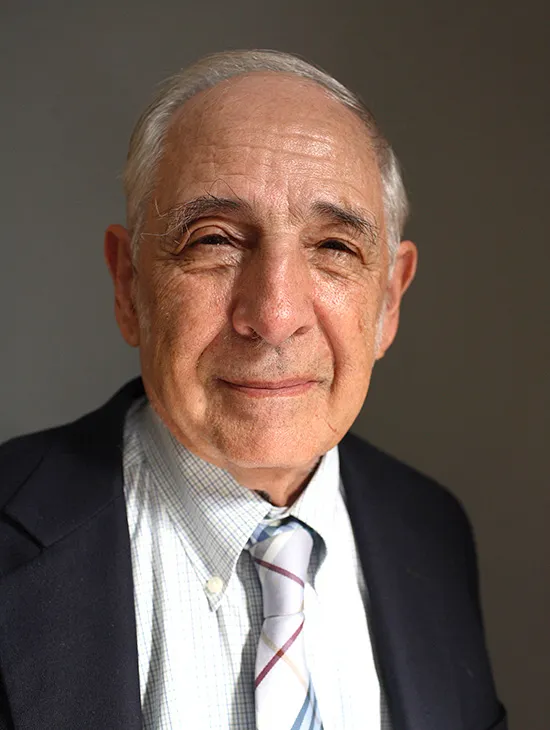
\includegraphics[width=.55\textwidth]{John-Searle.png}
				{\tiny\\John Searle\\\textit{\textcopyright Encyclopædia Britannica}}
			\end{figure}
		\end{minipage}
		\onslide<4->
		\begin{center}
			\hyperlink{subsec:turing_test}{\color{venis-faithful-yellow}\faExternalLinkSquare\ Indietro} o \href{https://plato.stanford.edu/entries/chinese-room/}{\faExternalLinkSquare\ Maggiori informazioni}
		\end{center}
	\end{minipage}
}
\end{frame}
%
\subsection{Convolutional Neural Networks}
\label{subsec:cnn}
%
\begin{frame}[t] \frametitle{Convolutional Neural Network (CNN)}
\framesubtitle{DL per Computer Vision}
{\footnotesize
\onslide<1->
	\begin{itemize}[leftmargin=10pt,align=right]
		\item[\alert{\faArrowCircleRight}] Nato come concetto algoritmico nel 1980
		\item[\alert{\faArrowCircleRight}] Insieme di architetture di reti neurali ottimizzata per \emph{task} su dati strutturati/gerarchici (es. \emph{image processing})
		\onslide<2->
		\item[\alert{\faArrowCircleRight}] Ricerca in piccoli gruppi di \emph{input} (\emph{\alert{pixel}}) caratteristiche locali (bordi, contorni, colori omogenei, $\ldots$)
		\onslide<3->
		\item[\alert{\faArrowCircleRight}] Strati sempre pi\'{u} profondi riconoscono \emph{features} (es. visuali) sempre pi\'{u} complesse
		\onslide<4->
		\begin{minipage}[t]{.8\textwidth}
			\begin{figure}[ht]
				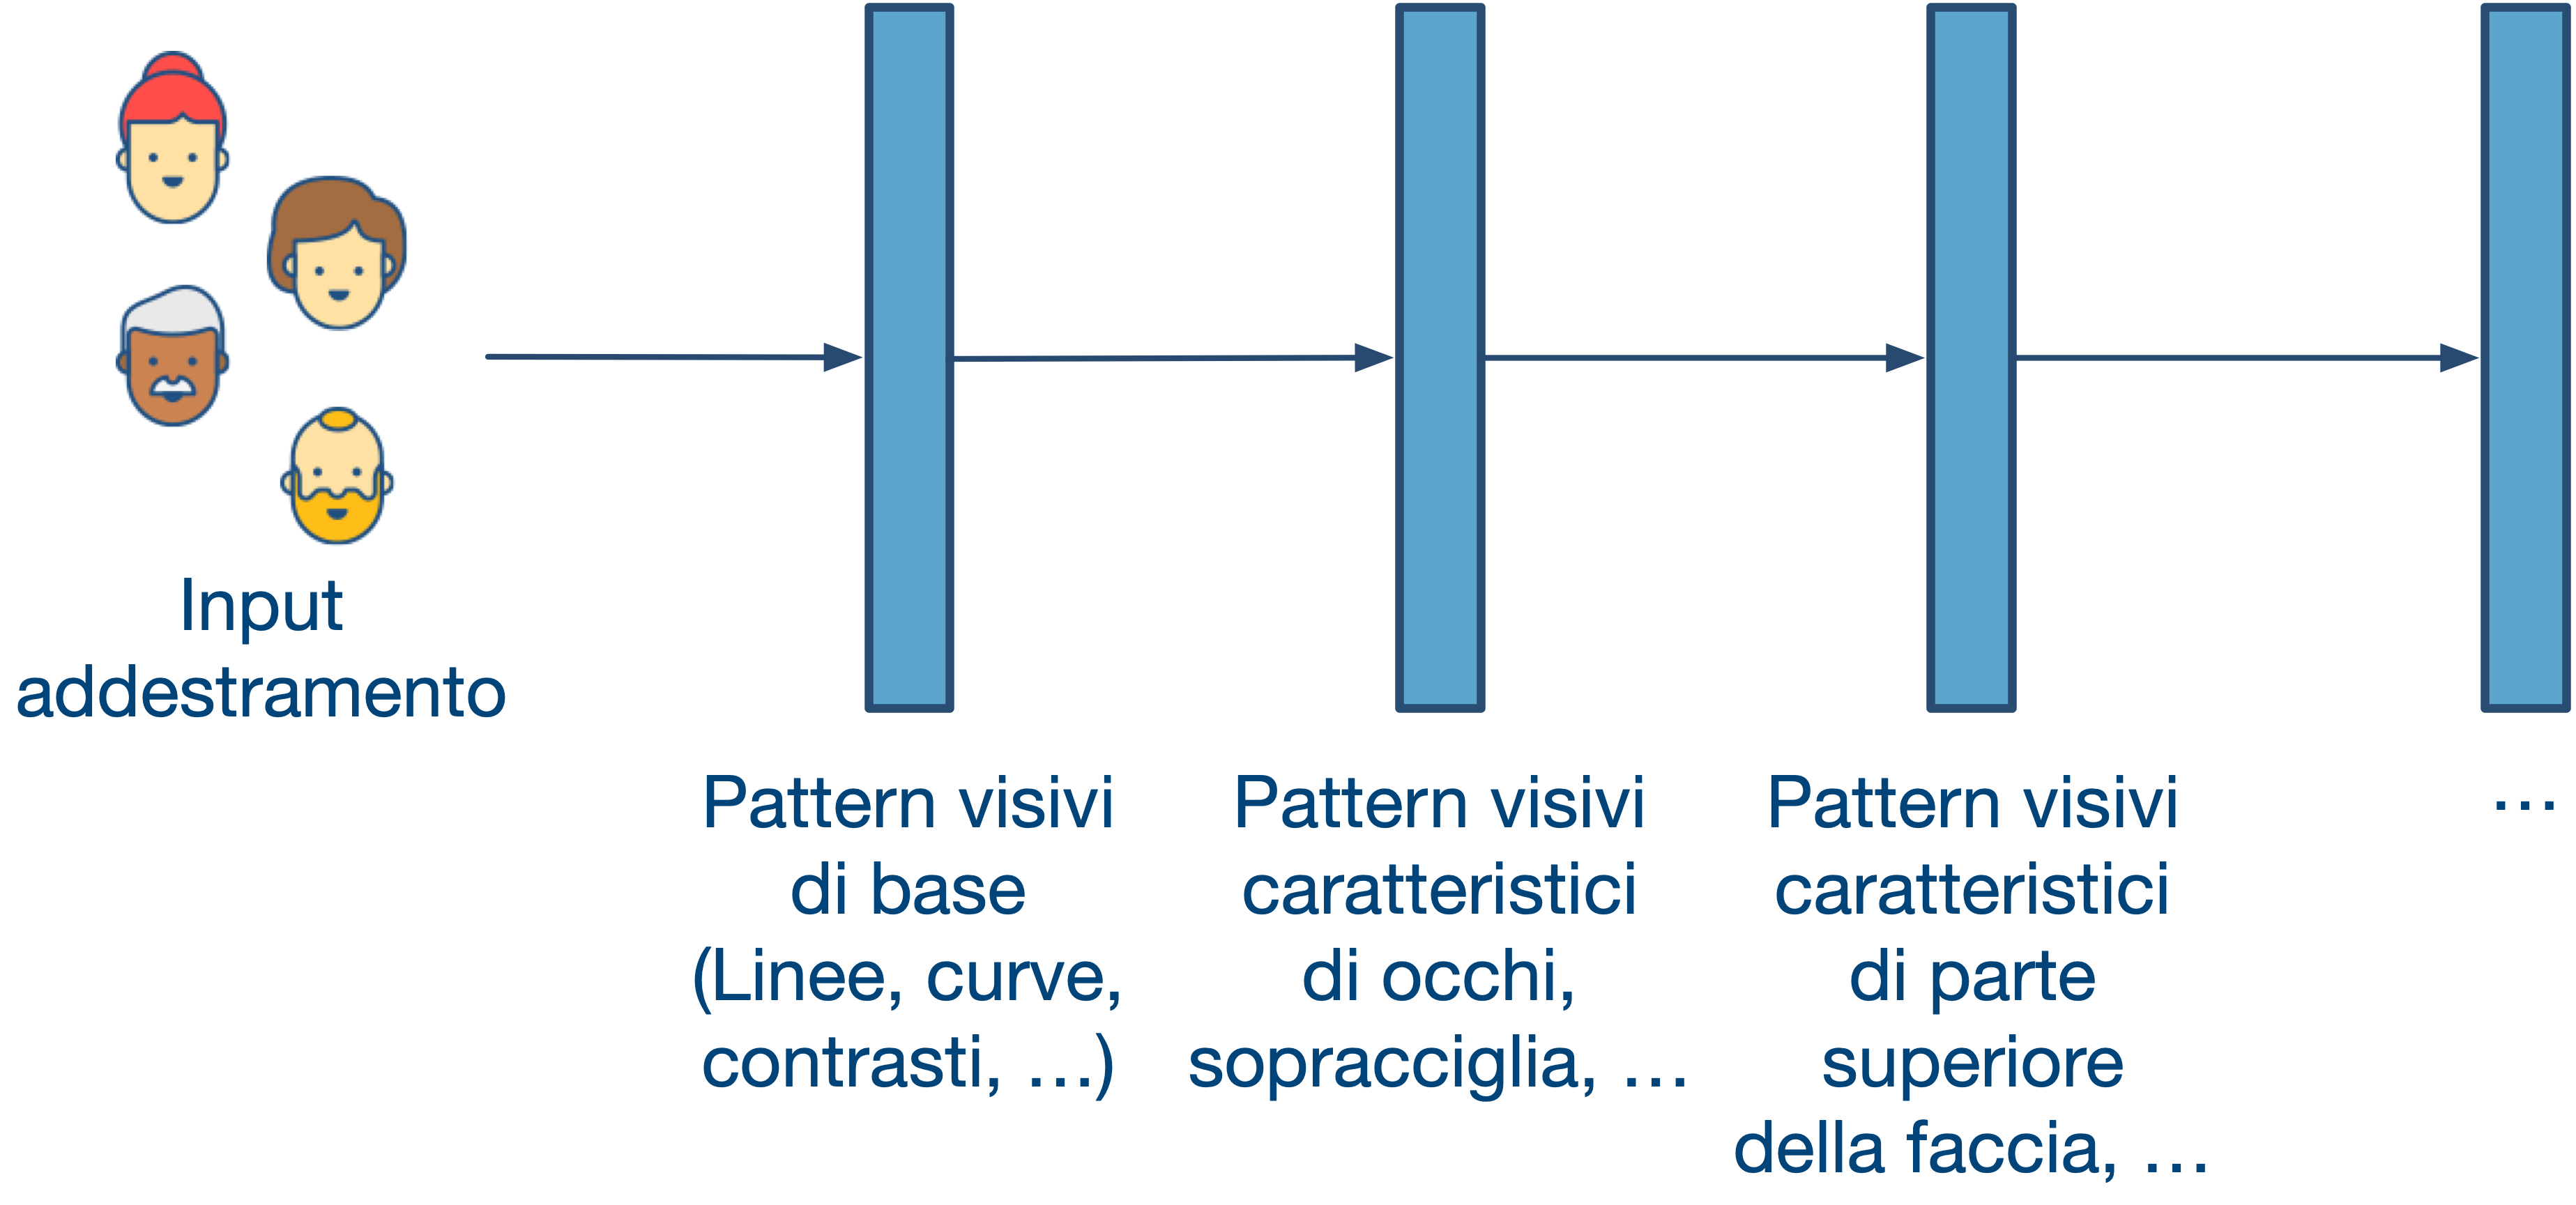
\includegraphics[width=.68\textwidth]{CNN-faces.png}
			\end{figure}
		\end{minipage}
		\onslide<5->
		\item[\alert{\faArrowCircleRight}] Funzioni di attivazione e tipologie di strati ispirati da
		\begin{itemize}[leftmargin=10pt,align=right]
			\item[\alert{\faArrowCircleRight}] Concetti biologici della corteccia visiva
			\item[\alert{\faArrowCircleRight}] Propriet\'{a} peculiari delle immagini
		\end{itemize}
	\end{itemize}
	\begin{center}
		\hyperlink{subsec:ai_rise}{\color{venis-faithful-yellow}\faExternalLinkSquare\ Indietro}
	\end{center}
}
\end{frame}